\section{About the EROS training set}

We use a training data set provided by \citet{kim2014} which contains labels (main and sub--classes) and lightcurves for $32655$ sources in the Large Magellanic Cloud (LMC). The lightcurves were recorded by the Expérience pour la Recherche d’Objets Sombres (EROS) project, a wide--field survey. A thorough description of the compilation process is available in \citet{kim2014}, however, here is a list of the main steps:

\begin{enumerate}
\item Compile known periodoic variables in the LMC from the OGLE and MACHO surveys
\item Add $982$ blue variables (BVs) from the MACHO database
\item Add 565 quasi--stellar objects (QSOs)
\item 
\end{enumerate}

% Number of sources in the data set
% Not a standard astronomical B and R bands

\section{Feature Extraction \& Feature Selection}

We extract a variety of features characterizing the variability of the source. A lot of them are standard statistical features, but some are more sophisticated, trying to incorporate a model of the underlying physics. In the following, $N$ will be the number of data points in the light curve, $(t_i, m_i)$ the $i^{\text{th}}$ data point in the light curve.

\begin{enumerate}
%\setlength{\itemsep}{5pt}
%\setlength{\parskip}{0pt}
%\setlength{\parsep}{0pt}
%\setlength{\abovedisplayskip}{.5em}
%\setlength{\belowdisplayskip}{.5em}

\litem{$\mu$ (Mean of magnitude)} The arithmetic mean of the magnitude, given by
\begin{equation}\mu = \frac{1}{N} \sum\limits_{i=1}^{N} m_i.\end{equation}

\litem{$\sigma$ (Standard deviation of magnitude)} The standard deviation of the magnitude, given by
\begin{equation}\sigma = \sqrt{\frac{1}{N} \sum_{i=1}^N (m_i - \mu)^2}.\end{equation}

\litem{$Q_{50}$ (Median of magnitude)} The median of the magnitude, given by
\begin{equation}Q_{50} = \cdots.\end{equation}

\litem{$\bar \mu$ (Weighted mean of magnitude)} The weighted arithmetic mean of the magnitude, given by
\begin{equation}\bar \mu = \big(\sum\limits_{i=1}^{N} w_i m_i\big) \; / \; \big(\sum\limits_{i=1}^{N} w_i\big).\end{equation}
% @TODO: Specify weights

\litem{$\bar \sigma$ (Weighted standard deviation of magnitude)} The weighted standard deviation of the magnitude, given by
\begin{equation}\bar \sigma = \cdots.\end{equation}
% @TODO: Specify weights
% @TODO: Add formula for weighted standard deviation

\litem{$\gamma_1$ (Skewness)} The skewness of the magnitude, given by
\begin{equation}\gamma_1 = \cdots.\end{equation}

\litem{$\gamma_2$ (Kurtosis)} The kurtosis of the magnitude, given by
\begin{equation}\gamma_2 = \cdots.\end{equation}

\litem{$Q_{25}$ (25\% quartile)} The 25\% quartile of the magnitude, given by
\begin{equation}Q_{25} = \cdots.\end{equation}

\litem{$Q_{75}$ (75\% quartile)} The 75\% quartile of the magnitude, given by
\begin{equation}Q_{75} = \cdots.\end{equation}

\litem{$\text{IQR}$ (Interquartile range)} The interquartile range of the magnitude, given by
\begin{equation}\text{IQR} = Q_{75} -Q_{25}.\end{equation}

\litem{$P_{\text{LS}}$ (Lomb--Scargle period)} The period of the signal according to the Lomb--Scargle algorithm, given by
\begin{equation}P_{\text{LS}} = \frac{1}{2 \sigma_y^2} \Bigg\{ \frac{\big[\sum\limits_{i=1}^k (y_i - \mu_y) \cos(\omega(t_i - \tau))\big]^2}{\sum\limits_{i=1}^k \cos^2(\omega(t_i - \tau))} + \frac{\big[\sum\limits_{i=1}^k (y_i - \mu_y) \sin(\omega(t_i - \tau))\big]^2}{\sum\limits_{i=1}^k \sin^2(\omega(t_i - \tau))}\Bigg\}\end{equation}

\litem{$\text{FAP}_{\text{LS}}$ (False--Alarm probability for Lomb--Scargle)} The false--alarm probability (FAP) for the Lomb--Scargle algorithm, given by
\begin{equation}\text{FAP}_{\text{LS}}(x) = 1 - (1 - \euler^{-x})^M.\end{equation}

\litem{$\text{SNR}$ (Signal--to--noise ratio)} The signal--to--noise ratio, given by
\begin{equation}\text{SNR} = \frac{\mu}{\sigma}.\end{equation}

\litem{$S$ (Shannon entropy)} The Shannon entropy of the signal, given by
\begin{equation}S = -\sum\limits_{i=1}^N m_i \ln(m_i).\end{equation}

\litem{$\eta$ ($\cdots$)} The $\eta$ feature as proposed by \citep{}, given by
\begin{equation}\eta = \frac{1}{\sigma^2 (N-1)} \sum\limits_{i=1}^{N-1} (m_{i+1} - m_{i})^2.\end{equation}

\litem{$\cdots$ (Half--magnitude--amplitude ratio)} The ratio between higher \resp lower amplitudes than average, given by
\begin{equation}\cdots = \cdots.\end{equation}

\litem{$\text{MAD}^{(1)}$ (Mean absolute deviation)} The mean absolute deviation of the magnitude, given by
\begin{equation}\text{MAD}^{(1)} = \cdots.\end{equation}

\litem{$\text{MAD}^{(2)}$ (Median absolute deviation)} The median absolute deviation of the magnitude, given by
\begin{equation}\text{MAD}^{(2)} = \cdots.\end{equation}

\litem{$\text{SF}_A$ (Structure function $A$)} The ...
\begin{equation}\text{SF}_A = \cdots.\end{equation}

\litem{$\text{SF}_\gamma$ (Structure function $\gamma$)} The ...
\begin{equation}\text{SF}_\gamma = \cdots.\end{equation}

\litem{$\mathcal{F}$ (Fourier series)} We fit standard fourier series with five terms to the phase--folded lightcurve.
\begin{equation}\mathcal{F}(t) = \frac{A_0}{2} + \sum_{k=1}^{\infty} ( A_k \cos(2 \pi k t) + B_k \sin(2 \pi k t) ).\end{equation}

% CE – three candidate periods + scores
% sf-A-error, sf-gamma-error
% Slope percentile features
% fourier-A-i, fourier-phi-i
% fourier-residuals

% Shapiro-W und Shapiro-p
% Proper citing of all equations

\end{enumerate}

This leads to a total of $\cdots$ features in $\cdots$ bands.

% State that feature are highly correlated
% Show histogram of some features.
% Show some scatterplots
% More about period finding

\section{Performance of the Support Vector Machine}

\begin{figure}[H]
\subfigure{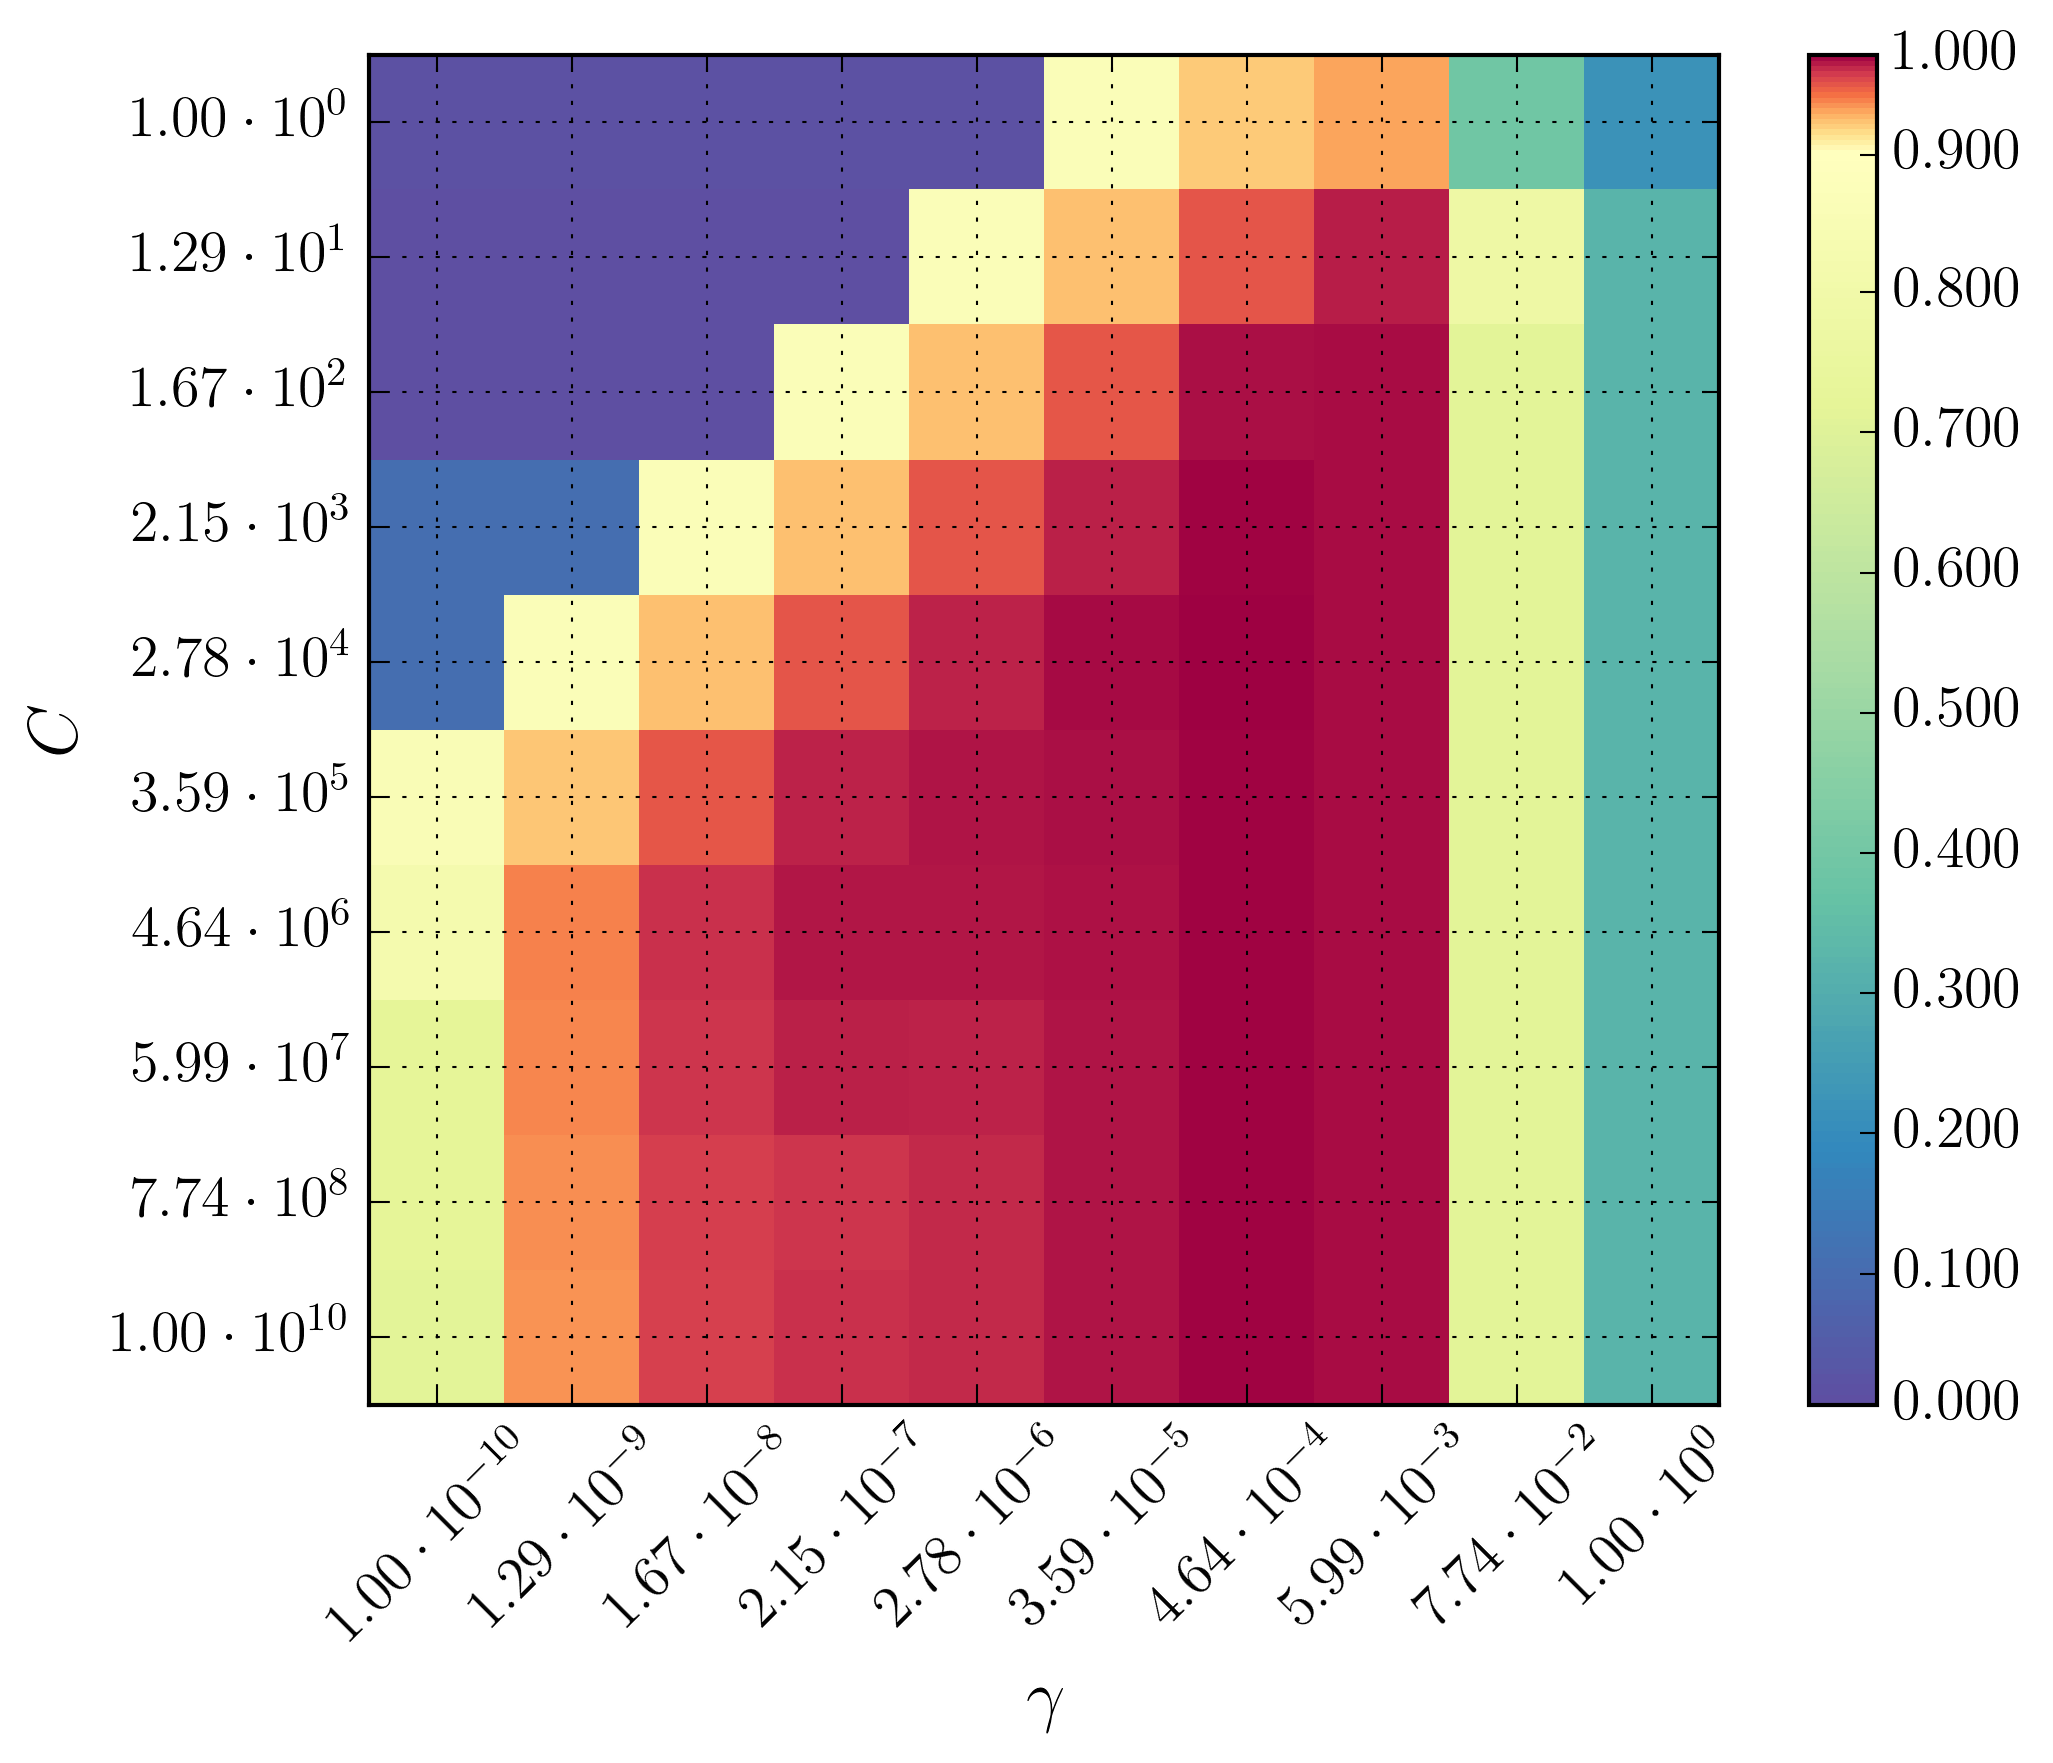
\includegraphics[width=0.49\textwidth,height=0.4\textwidth]{figures/gridsearch/svm/superclasses/svm-superclasses-01.png}}
\hfill
\subfigure{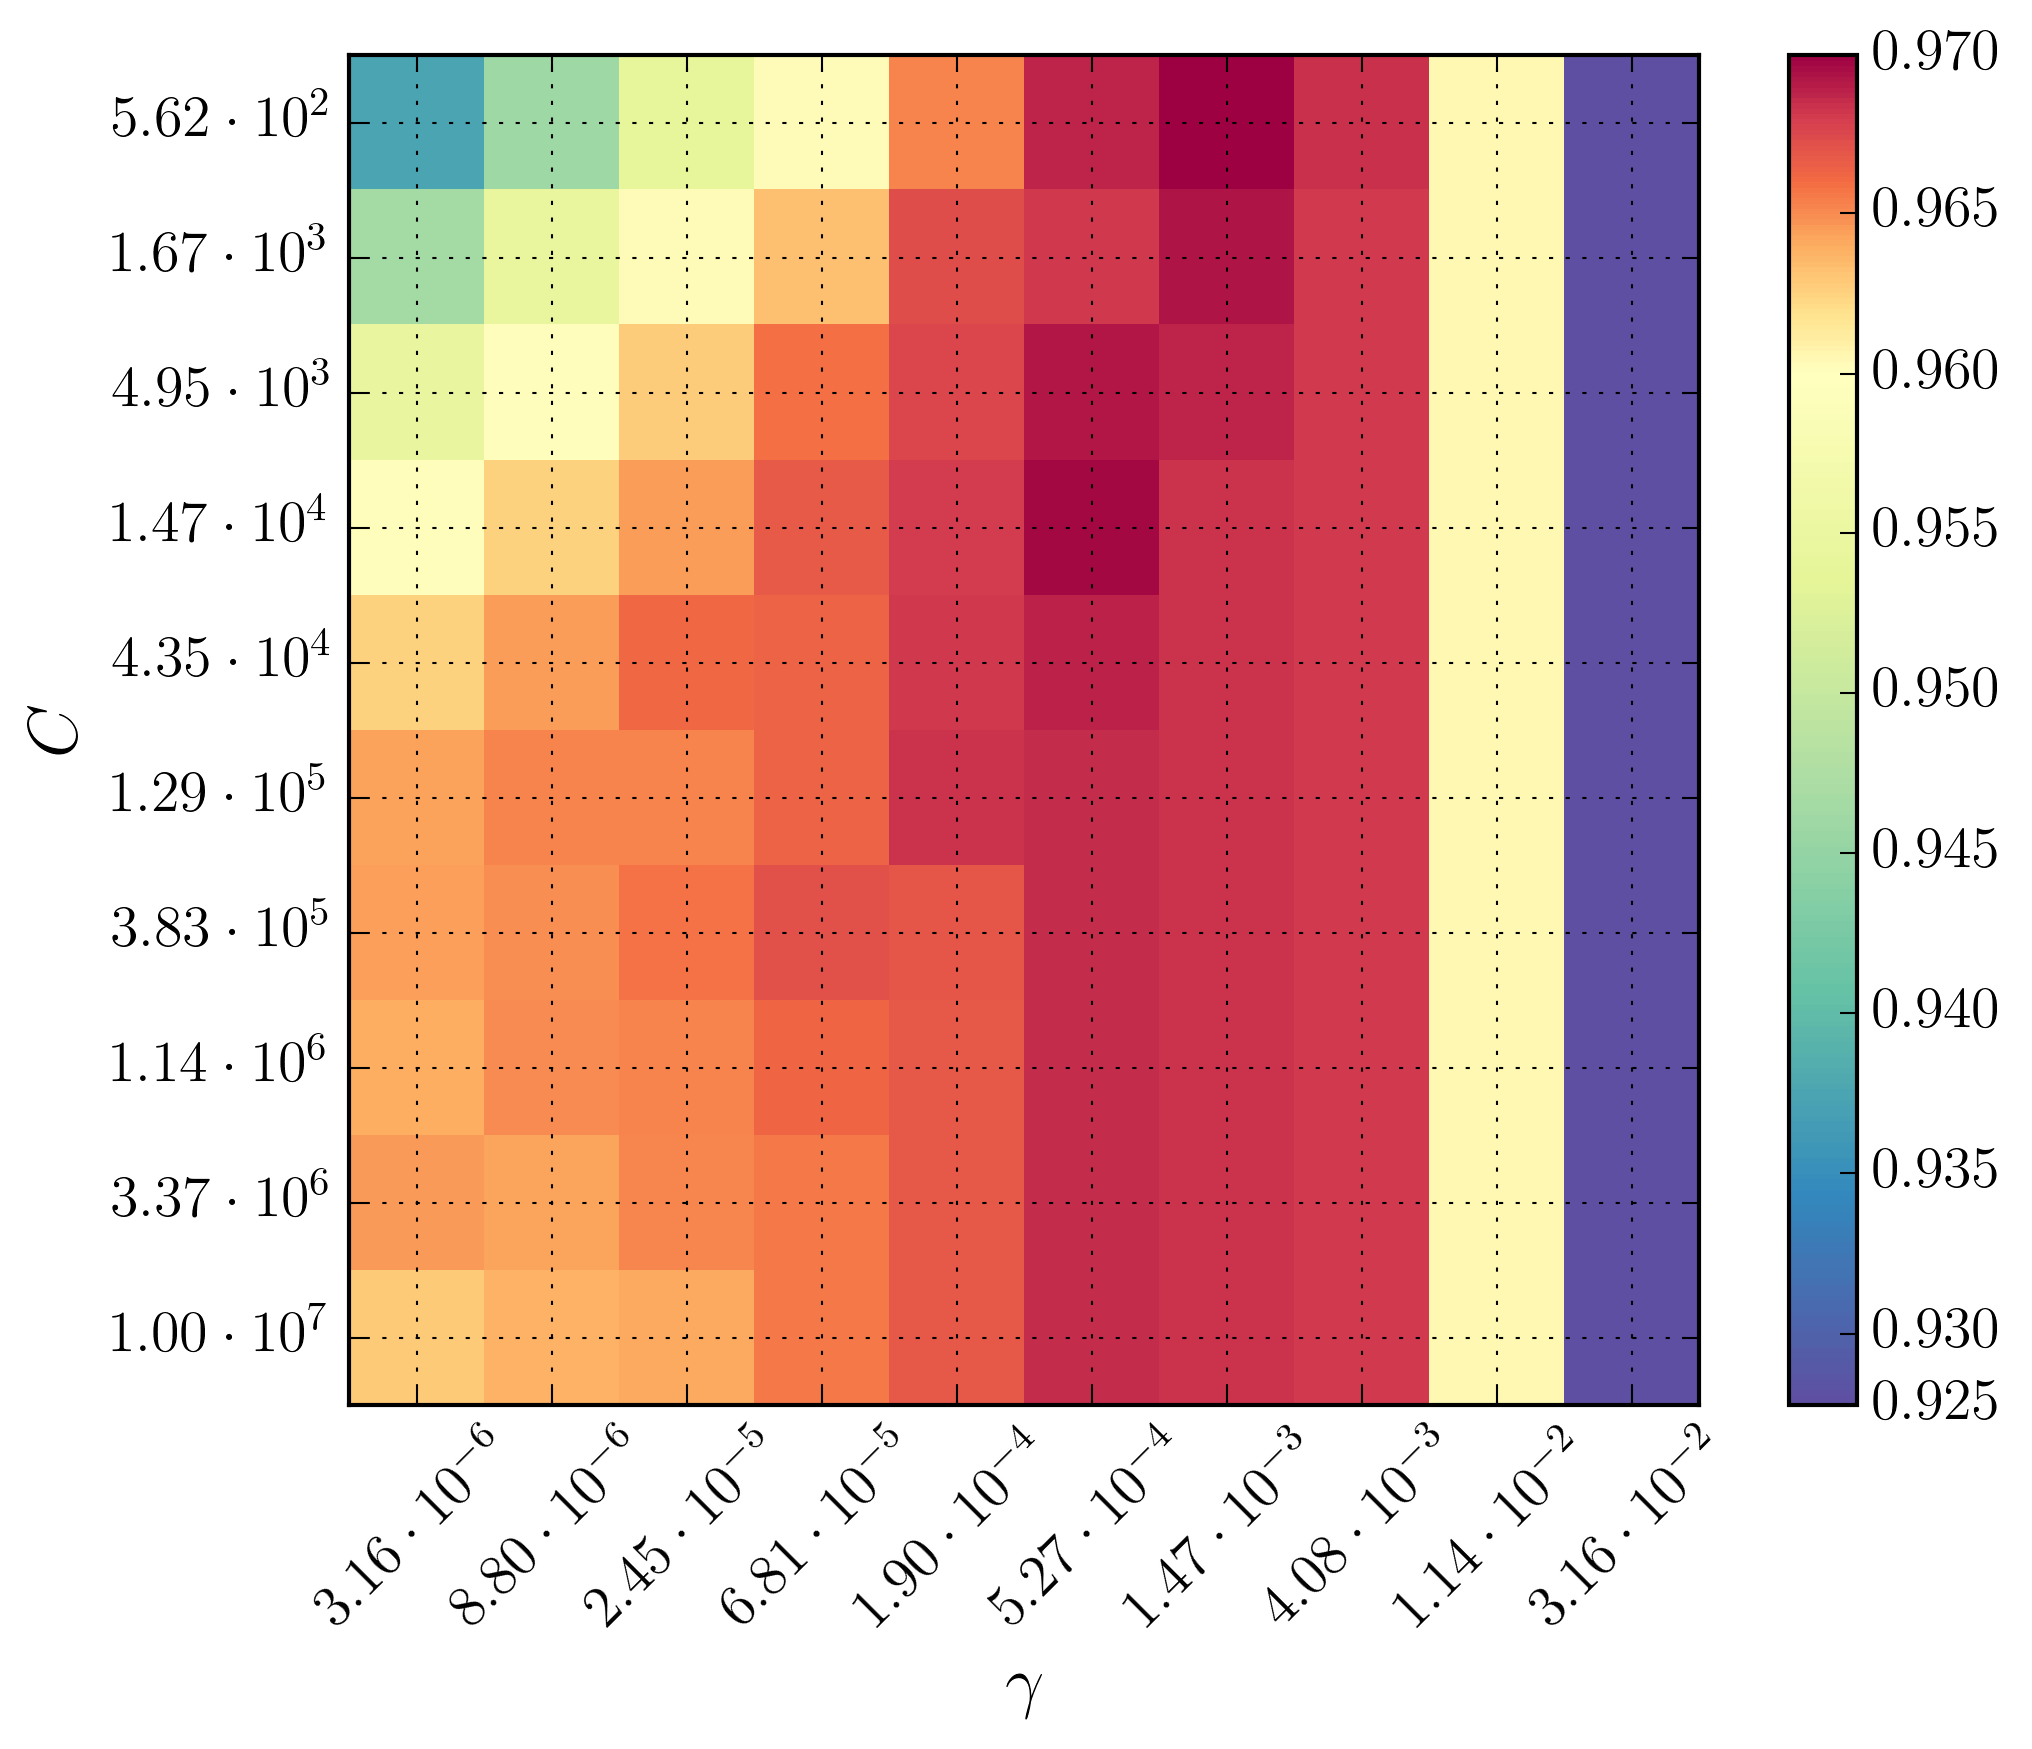
\includegraphics[width=0.51\textwidth,height=0.4\textwidth]{figures/gridsearch/svm/superclasses/svm-superclasses-02.png}}
\hfill
\subfigure{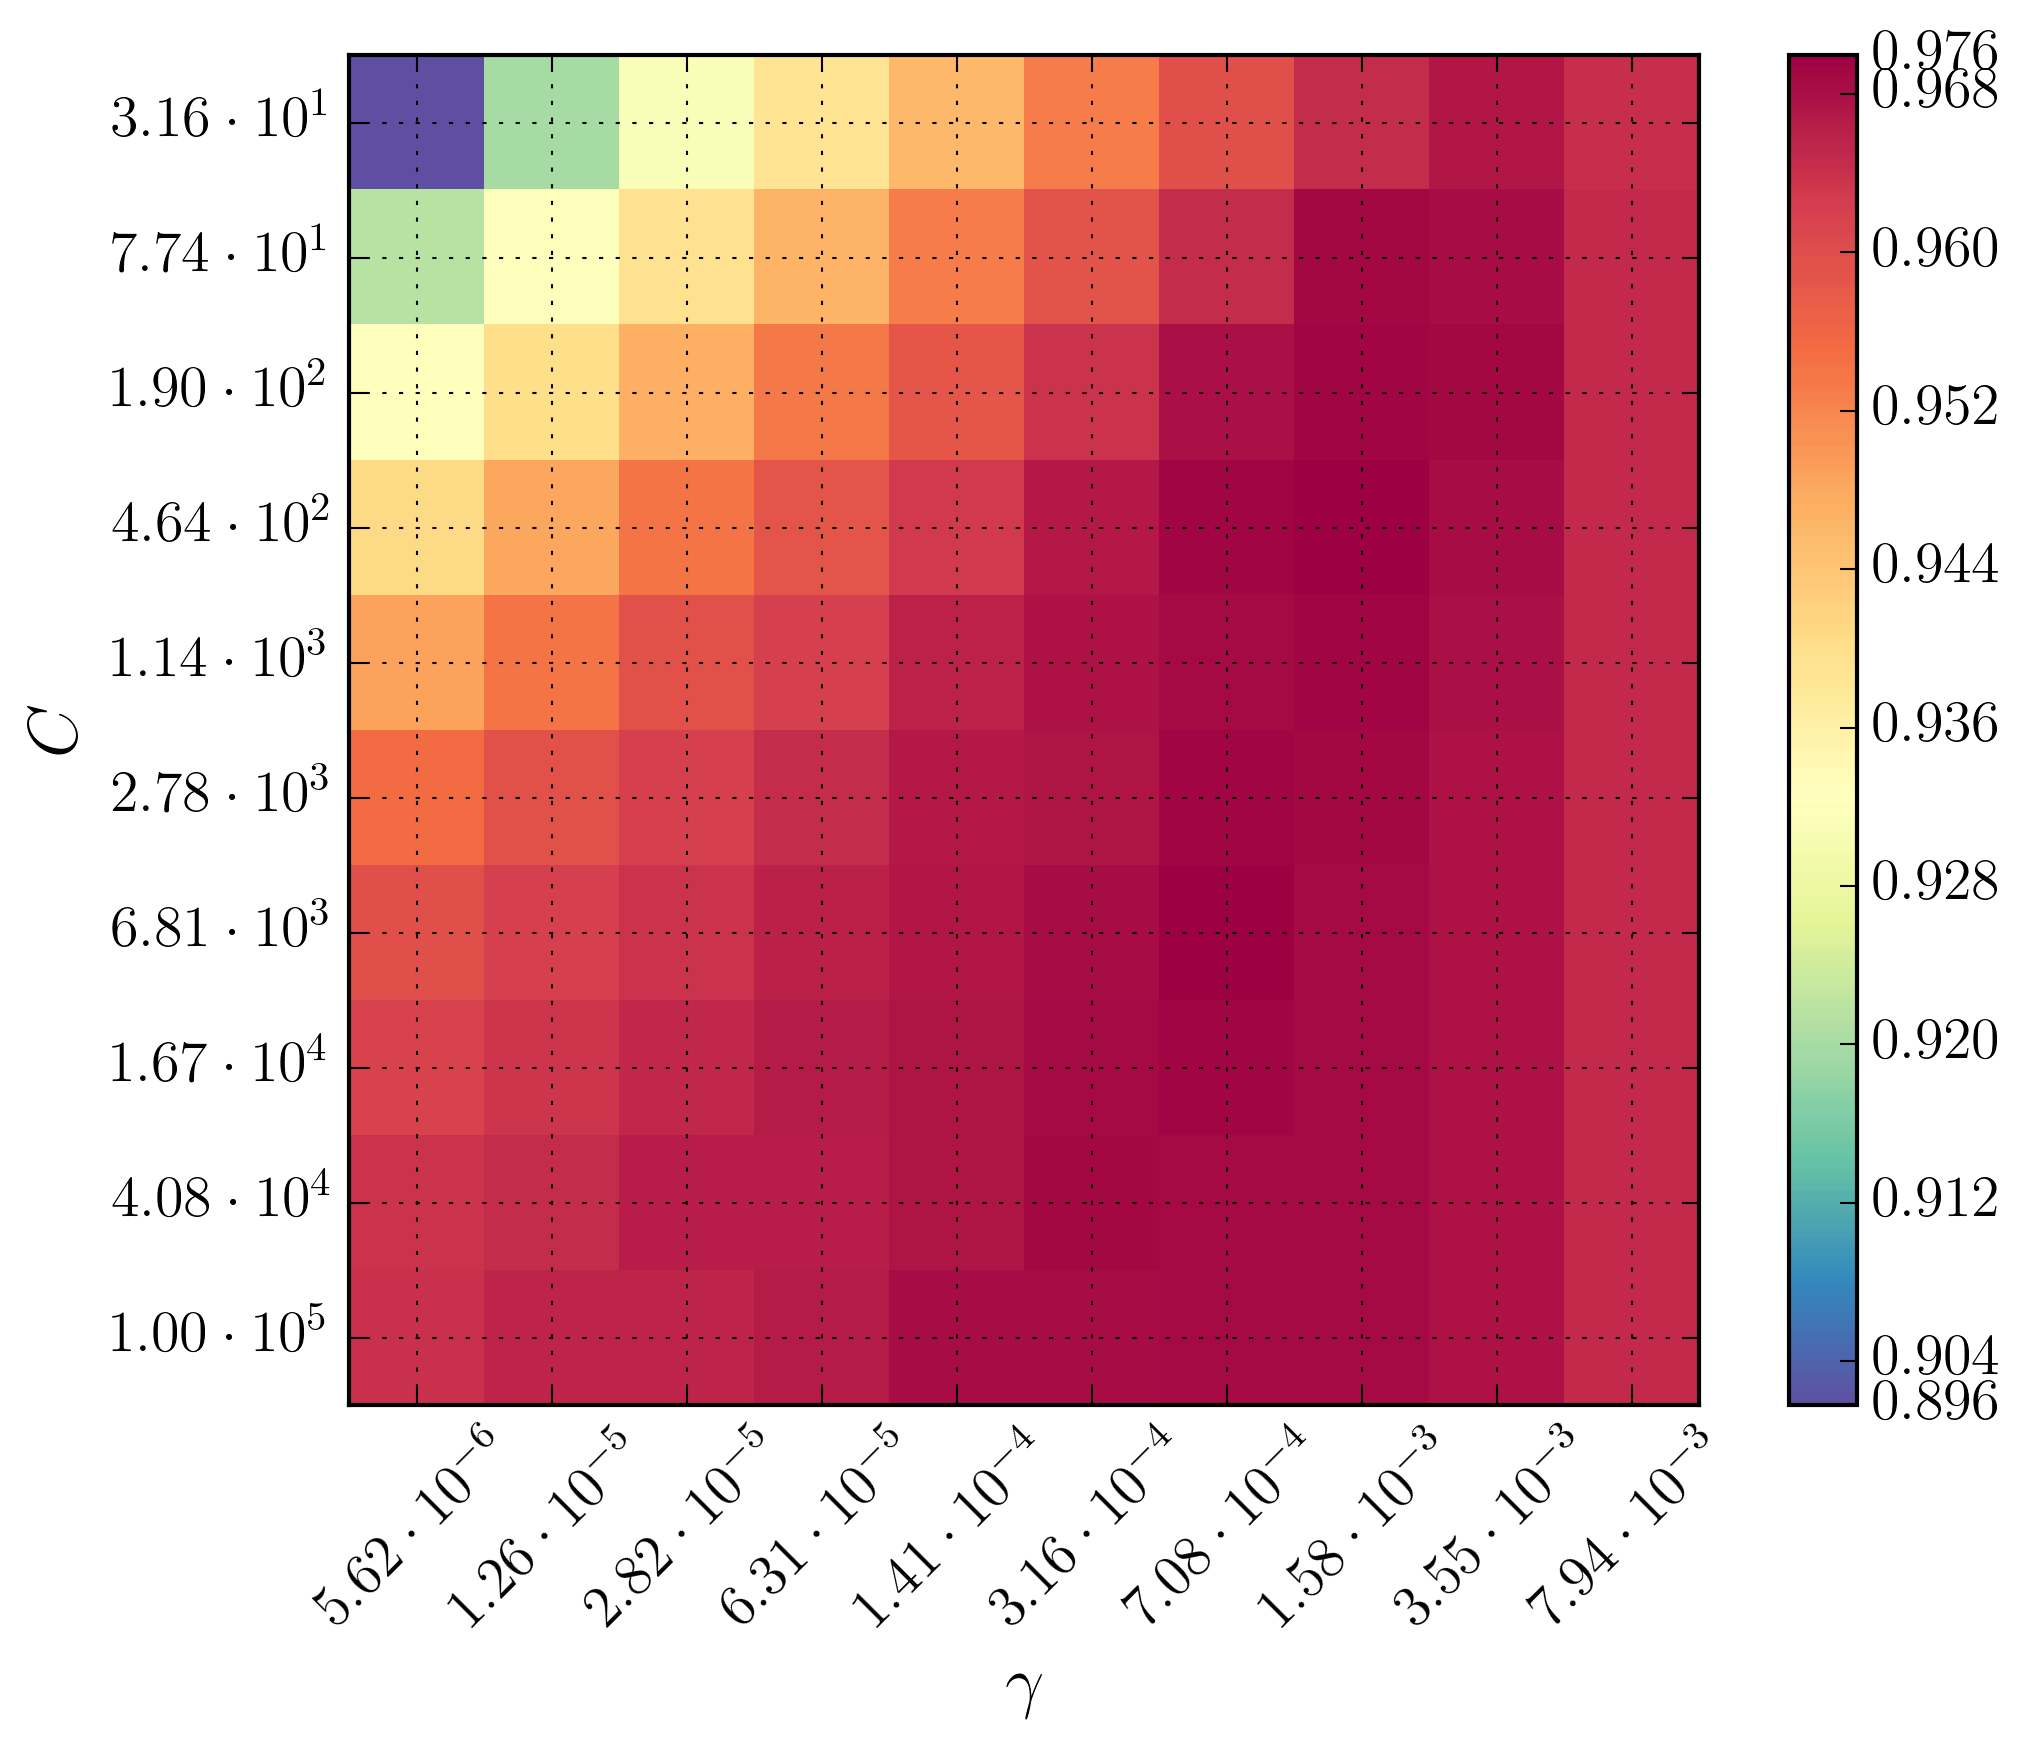
\includegraphics[width=0.49\textwidth,height=0.4\textwidth]{figures/gridsearch/svm/superclasses/svm-superclasses-03.png}}
\hfill
\subfigure{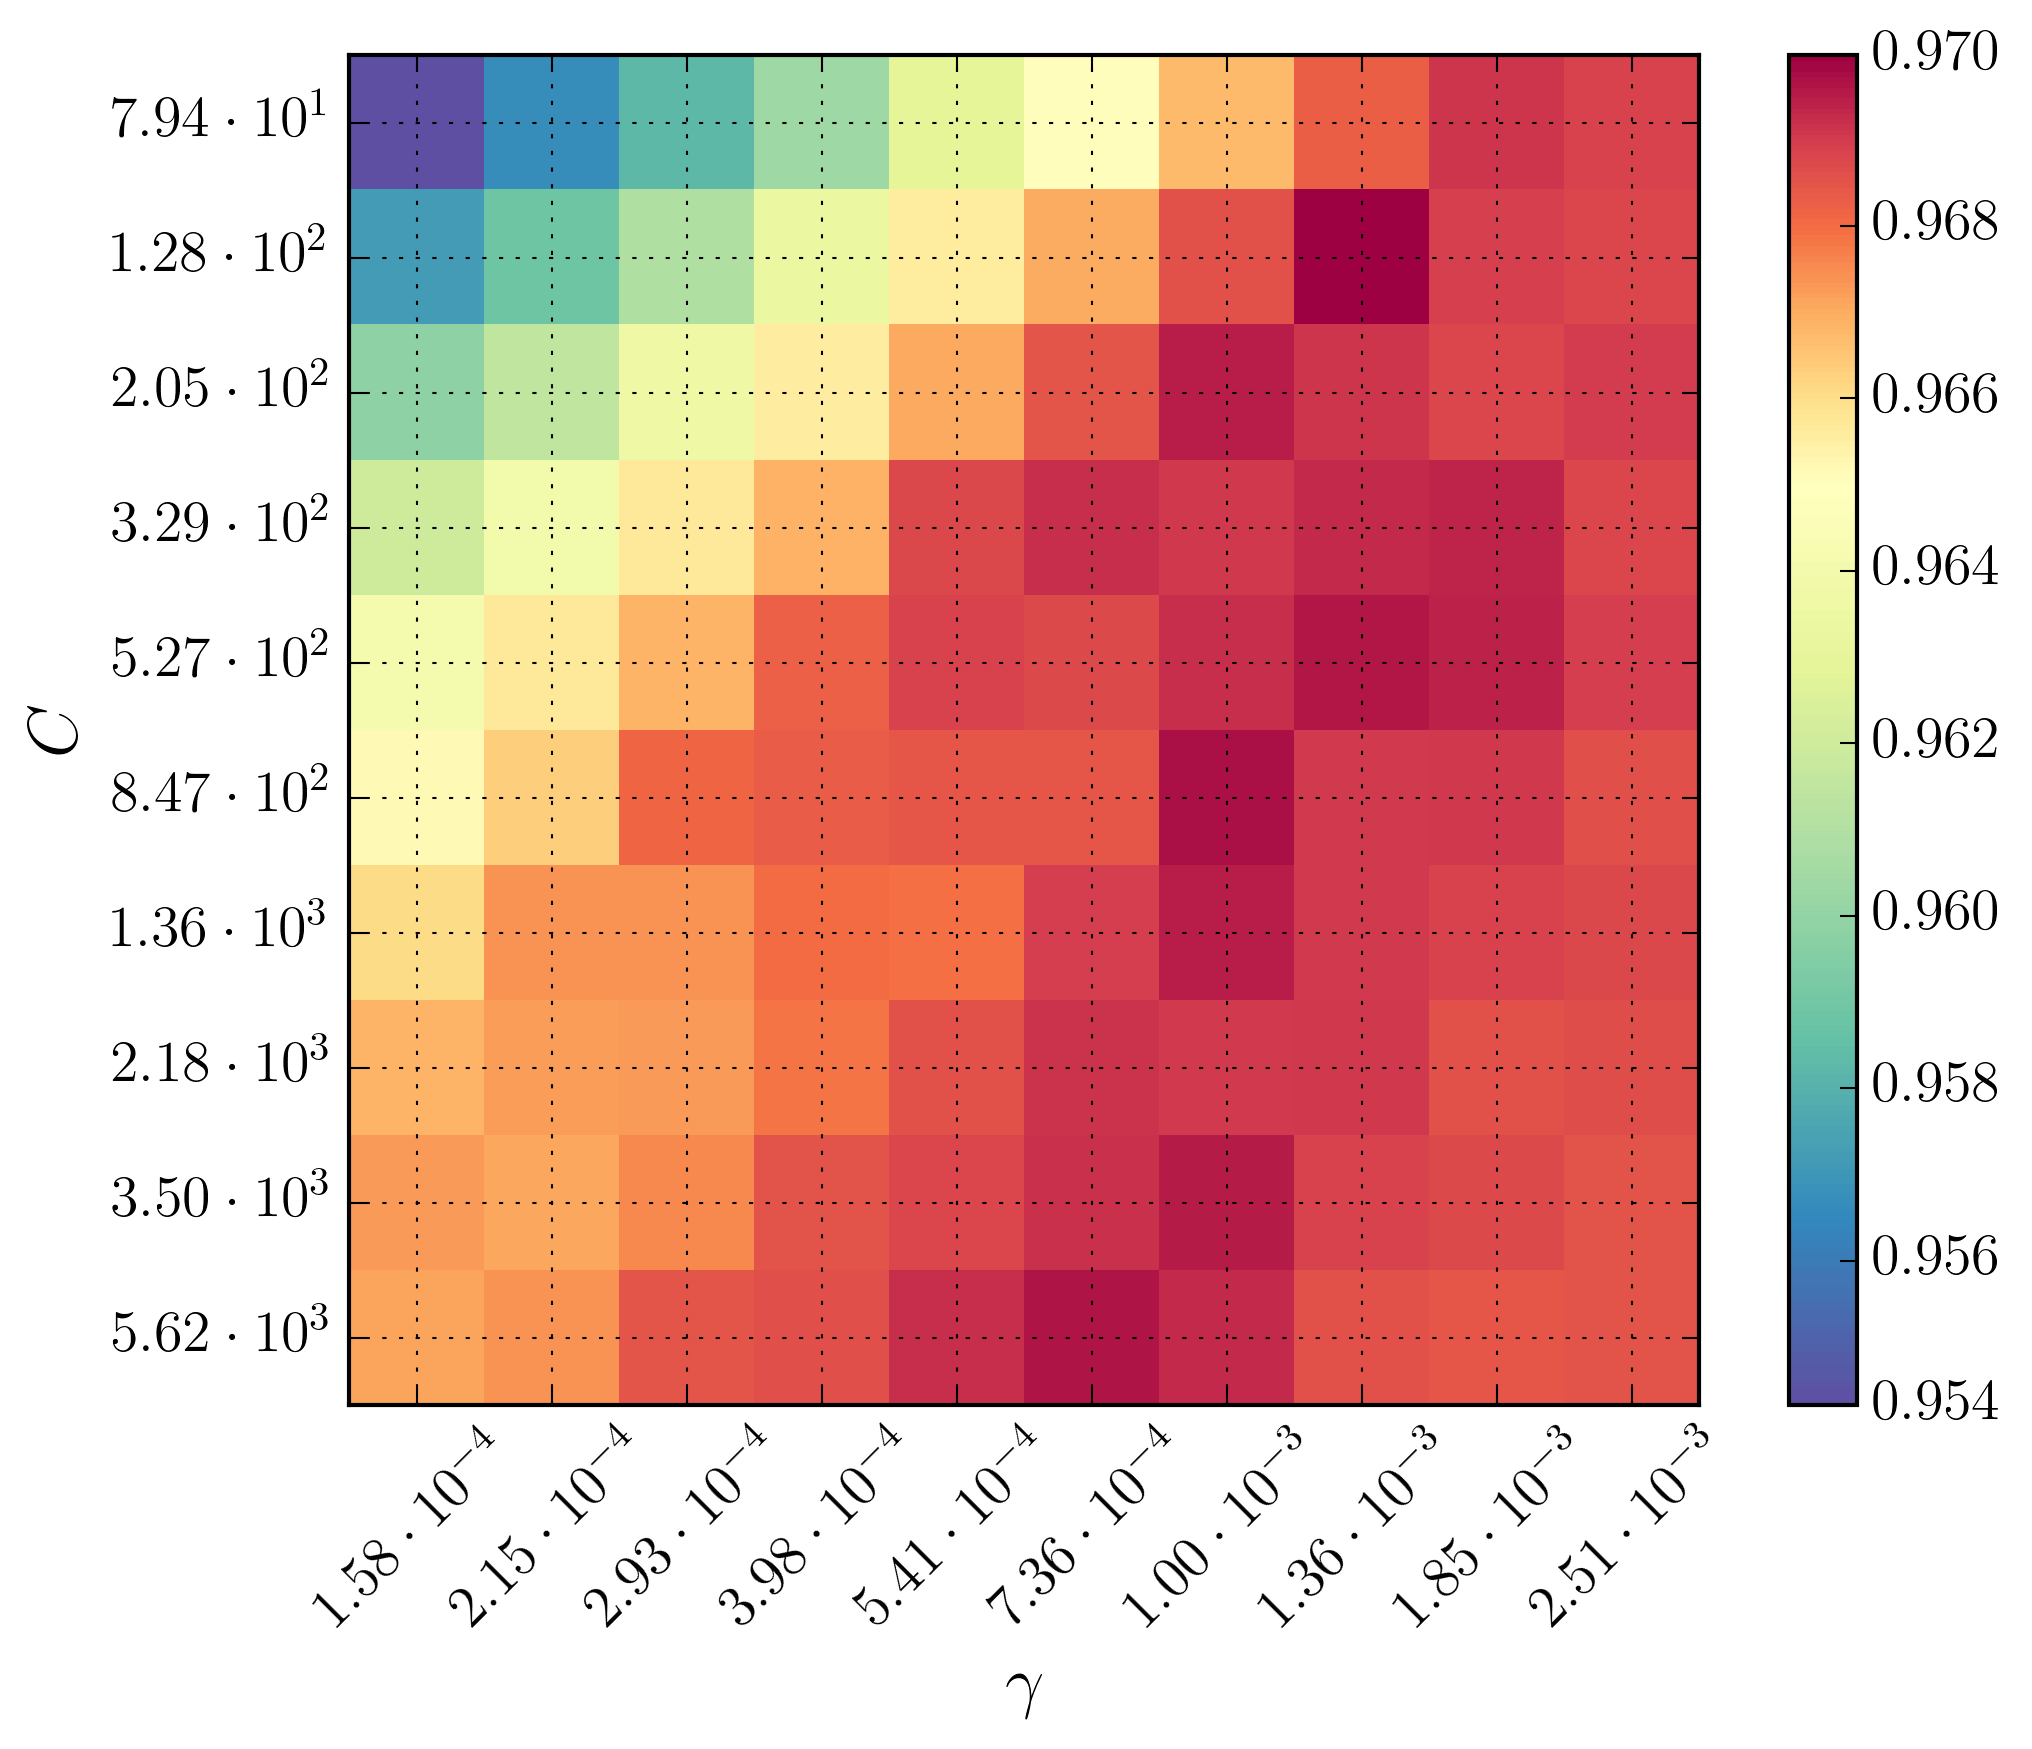
\includegraphics[width=0.51\textwidth,height=0.4\textwidth]{figures/gridsearch/svm/superclasses/svm-superclasses-04.png}}
\hfill
\subfigure{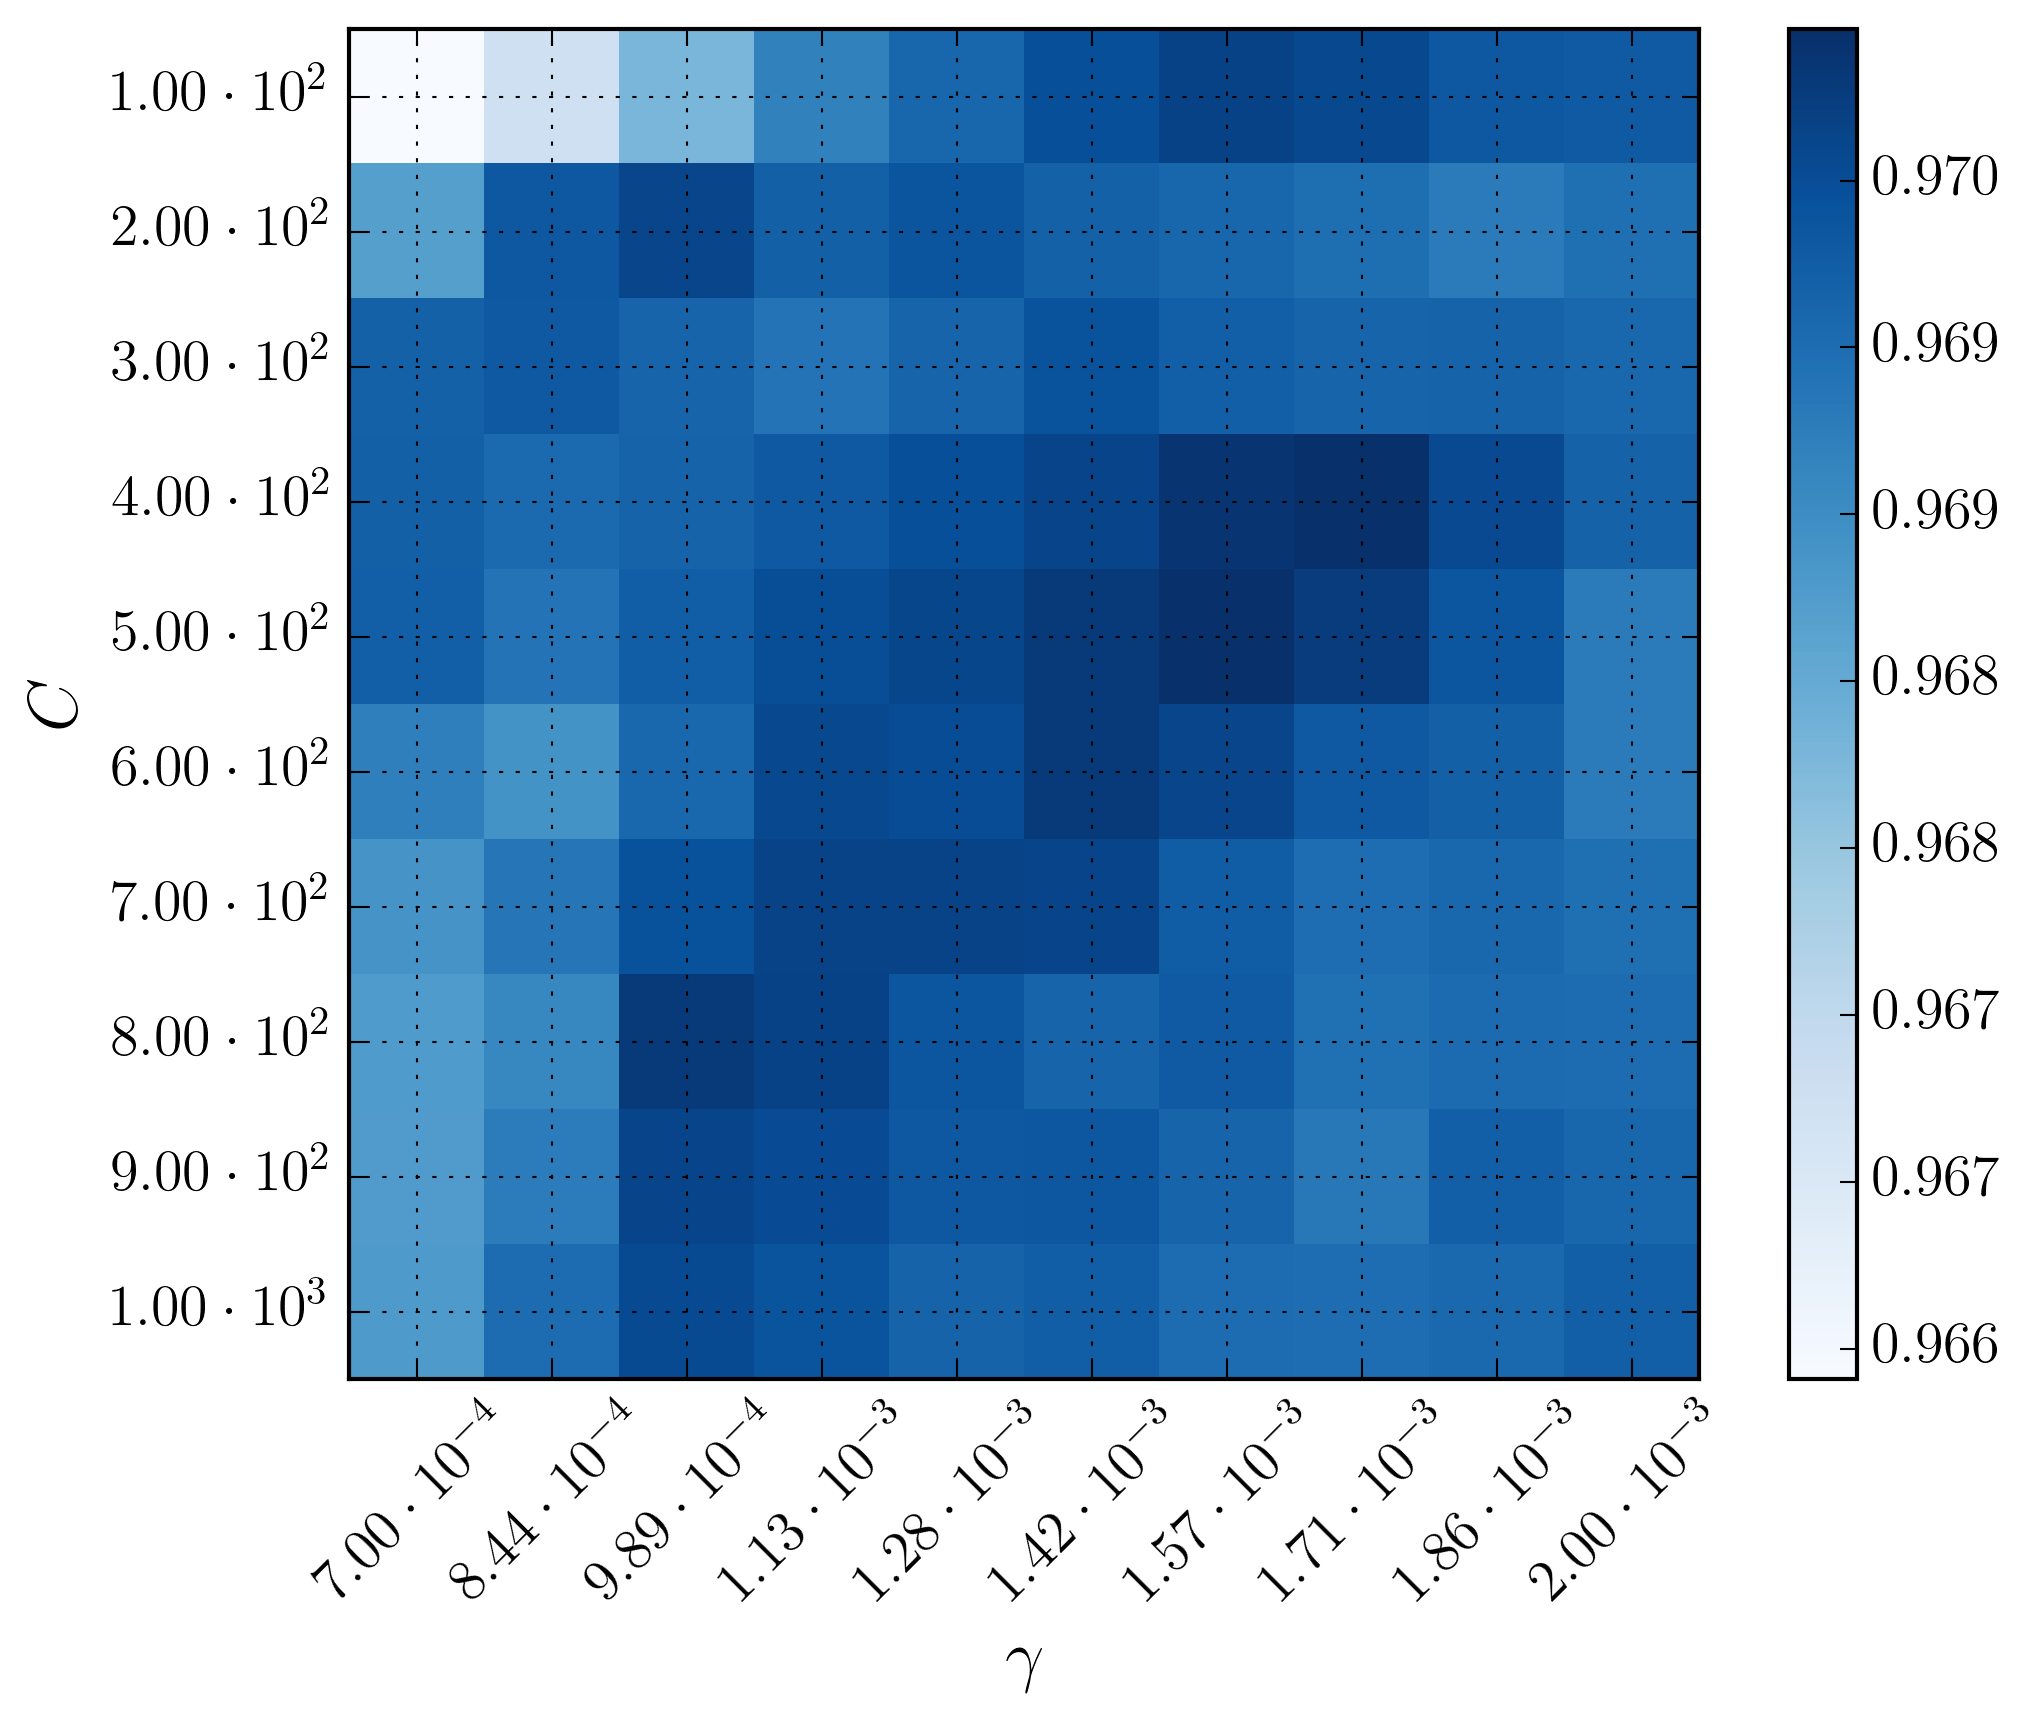
\includegraphics[width=0.49\textwidth,height=0.4\textwidth]{figures/gridsearch/svm/superclasses/svm-superclasses-05.png}}
\hfill
\subfigure{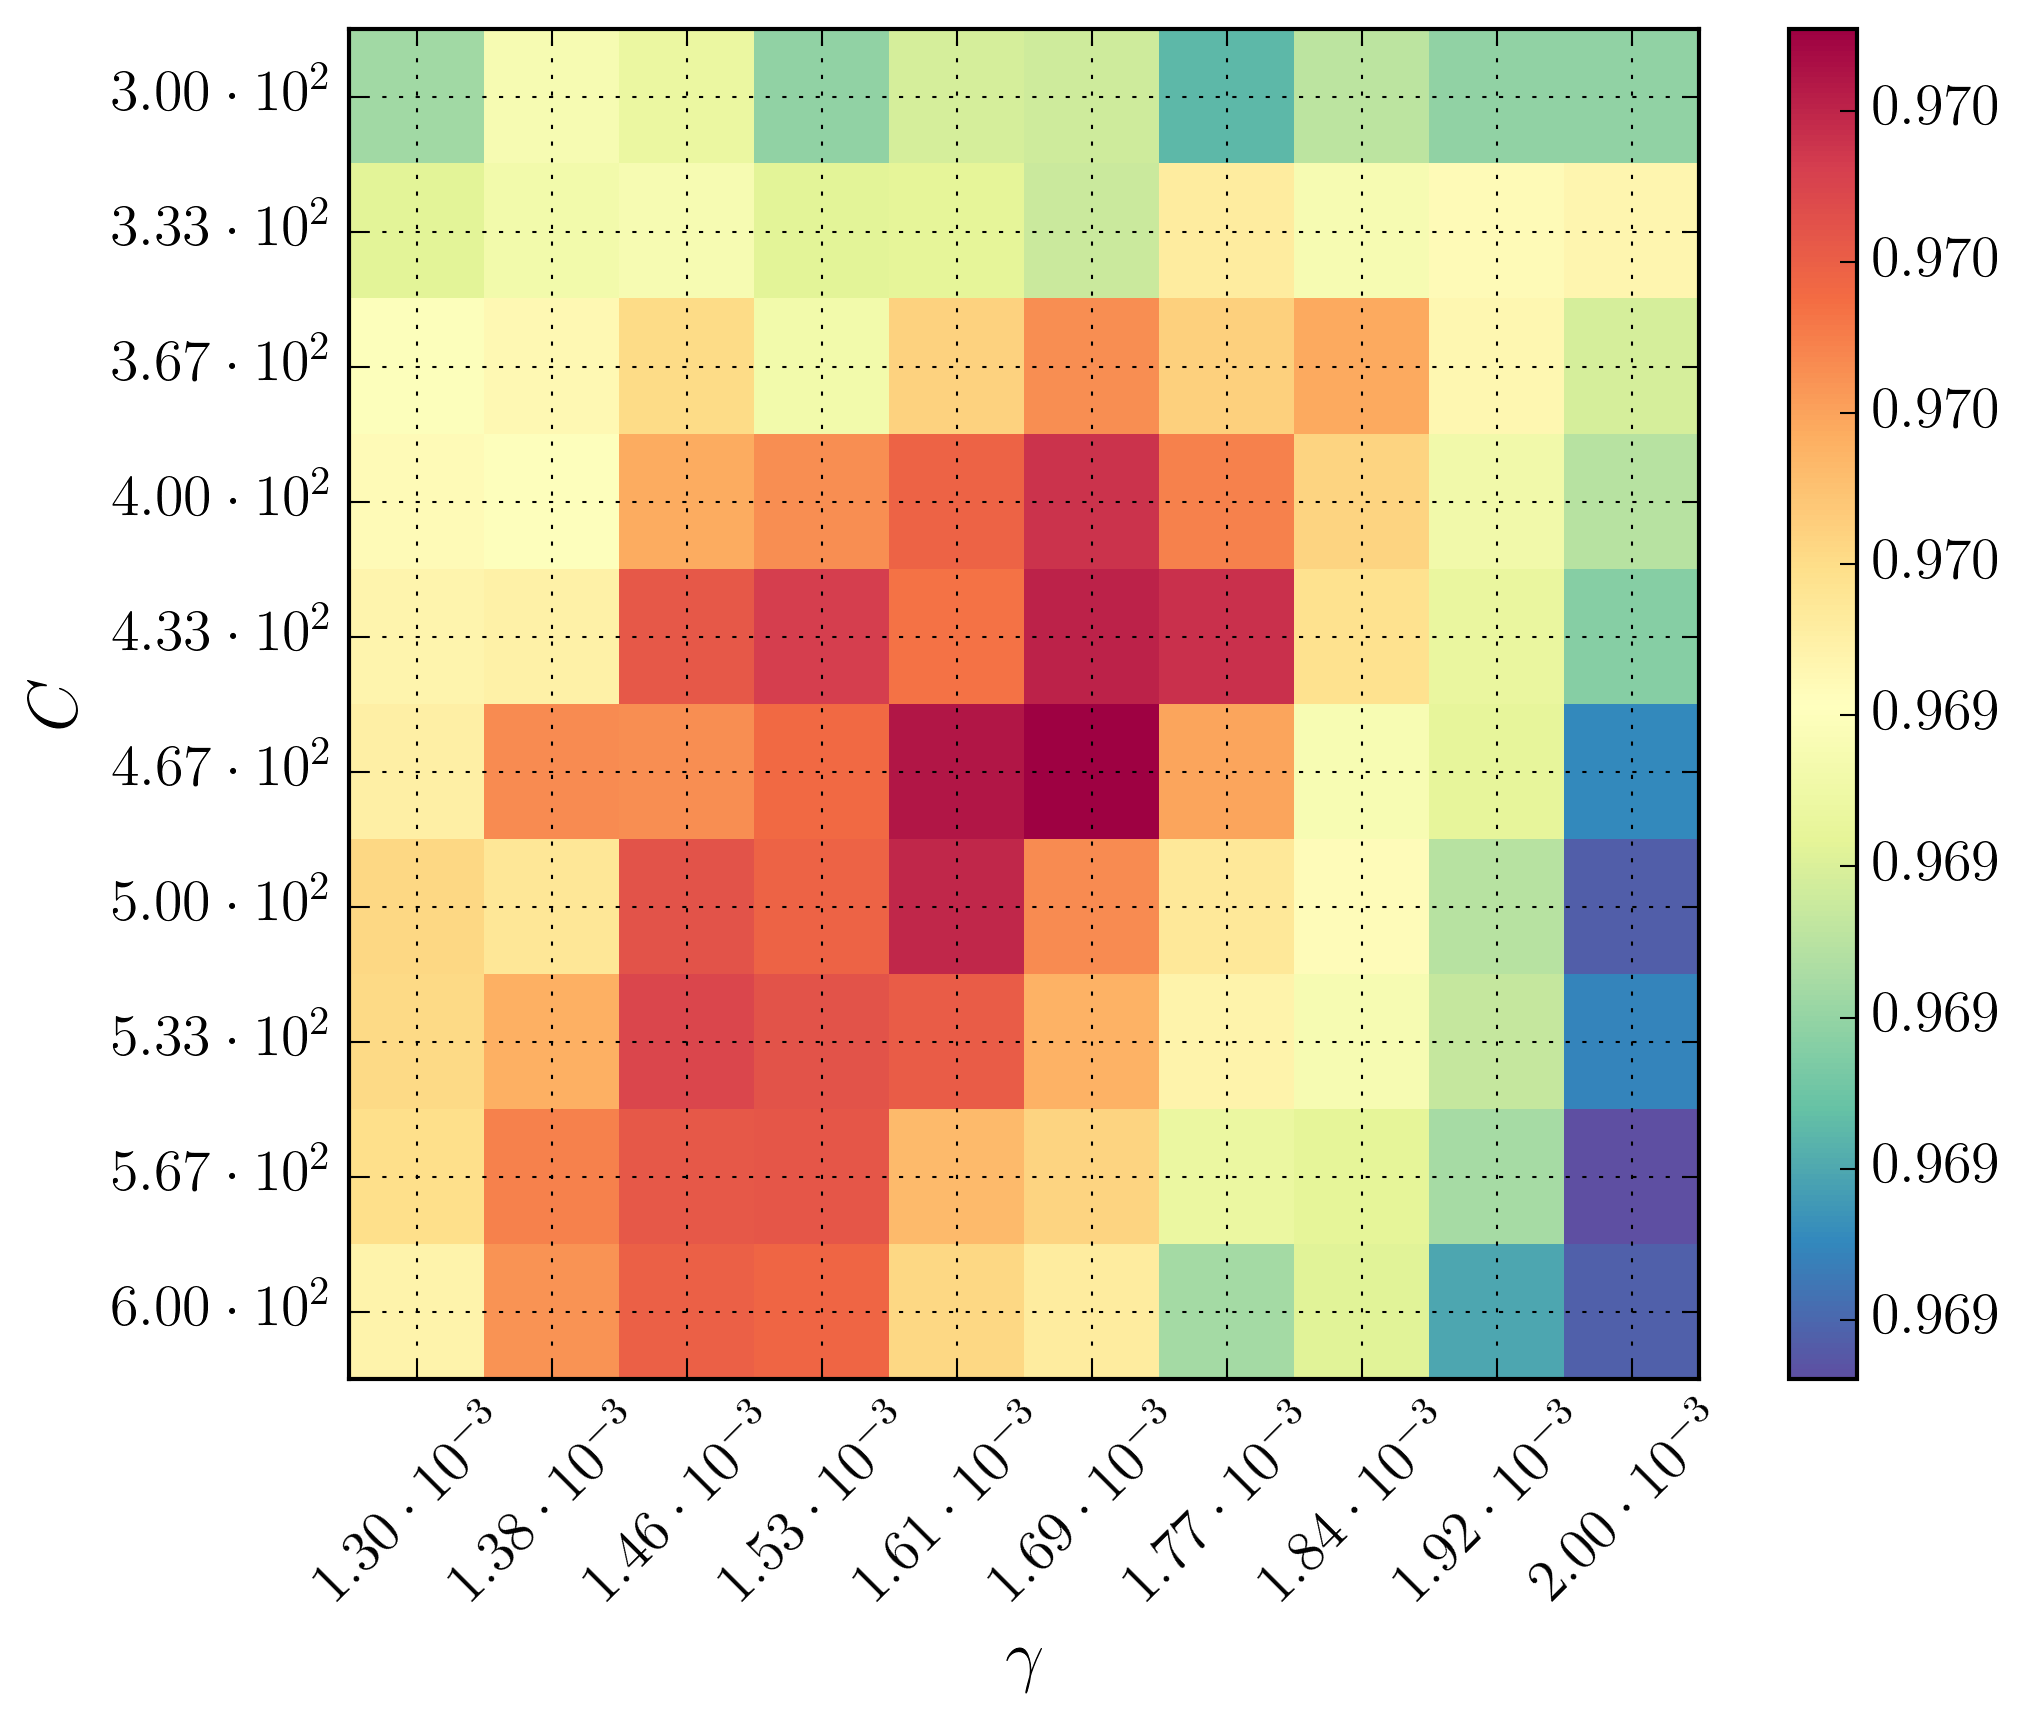
\includegraphics[width=0.51\textwidth,height=0.4\textwidth]{figures/gridsearch/svm/superclasses/svm-superclasses-06.png}}
\hfill
\caption[Hyperparameter optimization for the Support Vector Machine (SVM)]{This figure shows the average, weighted $F_1$ score on the $C$-$\gamma$-plane during the hyperparameter optimization for the Support Vector Machine. We start looking for global optima on a coarse grid with a wide range (upper left), and adjust the grid toward a finer stepwidth. At some point we find an optimum (lower right).}
\label{fig:gridsearch-svm-superclasses}
\end{figure}

% Hyperparameter optimization
% Add confusion matrix for main classes
% Add confusion matrix for subclasses

\renewcommand{\arraystretch}{1.5}
\resizebox{\textwidth}{!}{
\begin{tabular}{c|ccccccccc|c}
\toprule
%& \multicolumn{8 }{c}{Predicted class} & & \\
%\hline
                   & BV        & CEPH       & DSCT      & EB         & LPV         & NoneVar    & QSO       & RRL        & T2CEPH   & $\Sigma $ \\
\hline
BV                 & {\bf 762} &            &           &     12     &     1       &     19     &      1    &            &     1    &     796   \\
CEPH               &     2     & {\bf 2218} &           &     13     &     5       &     3      &           &     28     &    12    &    2281   \\
DSCT               &           &      5     & {\bf 453} &     8      &             &     17     &           &     28     &          &     511   \\
EB                 &    16     &      16    &     10    & {\bf 3336} &     50      &     54     &      5    &     46     &     5    &    3538   \\
LPV                &     5     &      5     &           &     46     & {\bf 15884} &     51     &      2    &     2      &          &   15995   \\
NoneVar            &    15     &      1     &     14    &     48     &     65      & {\bf 4621} &      24   &     3      &          &    4791   \\
QSO                &     2     &      1     &           &     1      &      1      &     30     & {\bf 144} &     1      &          &     180   \\
RRL                &           &      27    &     34    &     60     &      4      &     7      &      0    & {\bf 4336} &     2    &    4470   \\
T2CEPH             &     1     &      23    &           &     16     &      6      &     1      &           &     11     & {\bf 63} &     121   \\
\bottomrule
Recall ($\%$)      &   95.73   &     97.24  &   88.65   &    94.29   &    99.31    &   96.45    &    80.00  &    97.00   &   52.07  &           \\
\hline
Precision ($\%$)   &   94.89   &     96.60  &   88.65   &    94.24   &    99.18    &   96.21    &    81.82  &    97.33   &   75.90  &           \\
\hline
$F_1$ score ($\%$) &   95.31   &     96.92  &   88.65   &    94.26   &    99.24    &   96.33    &    80.90  &    97.16   &   61.77  & 97.25 $\pm$ 0.25 \\
\bottomrule
\end{tabular}
}

\section{Performance of the Random Forest Classifier}

\begin{figure}[H]
\subfigure{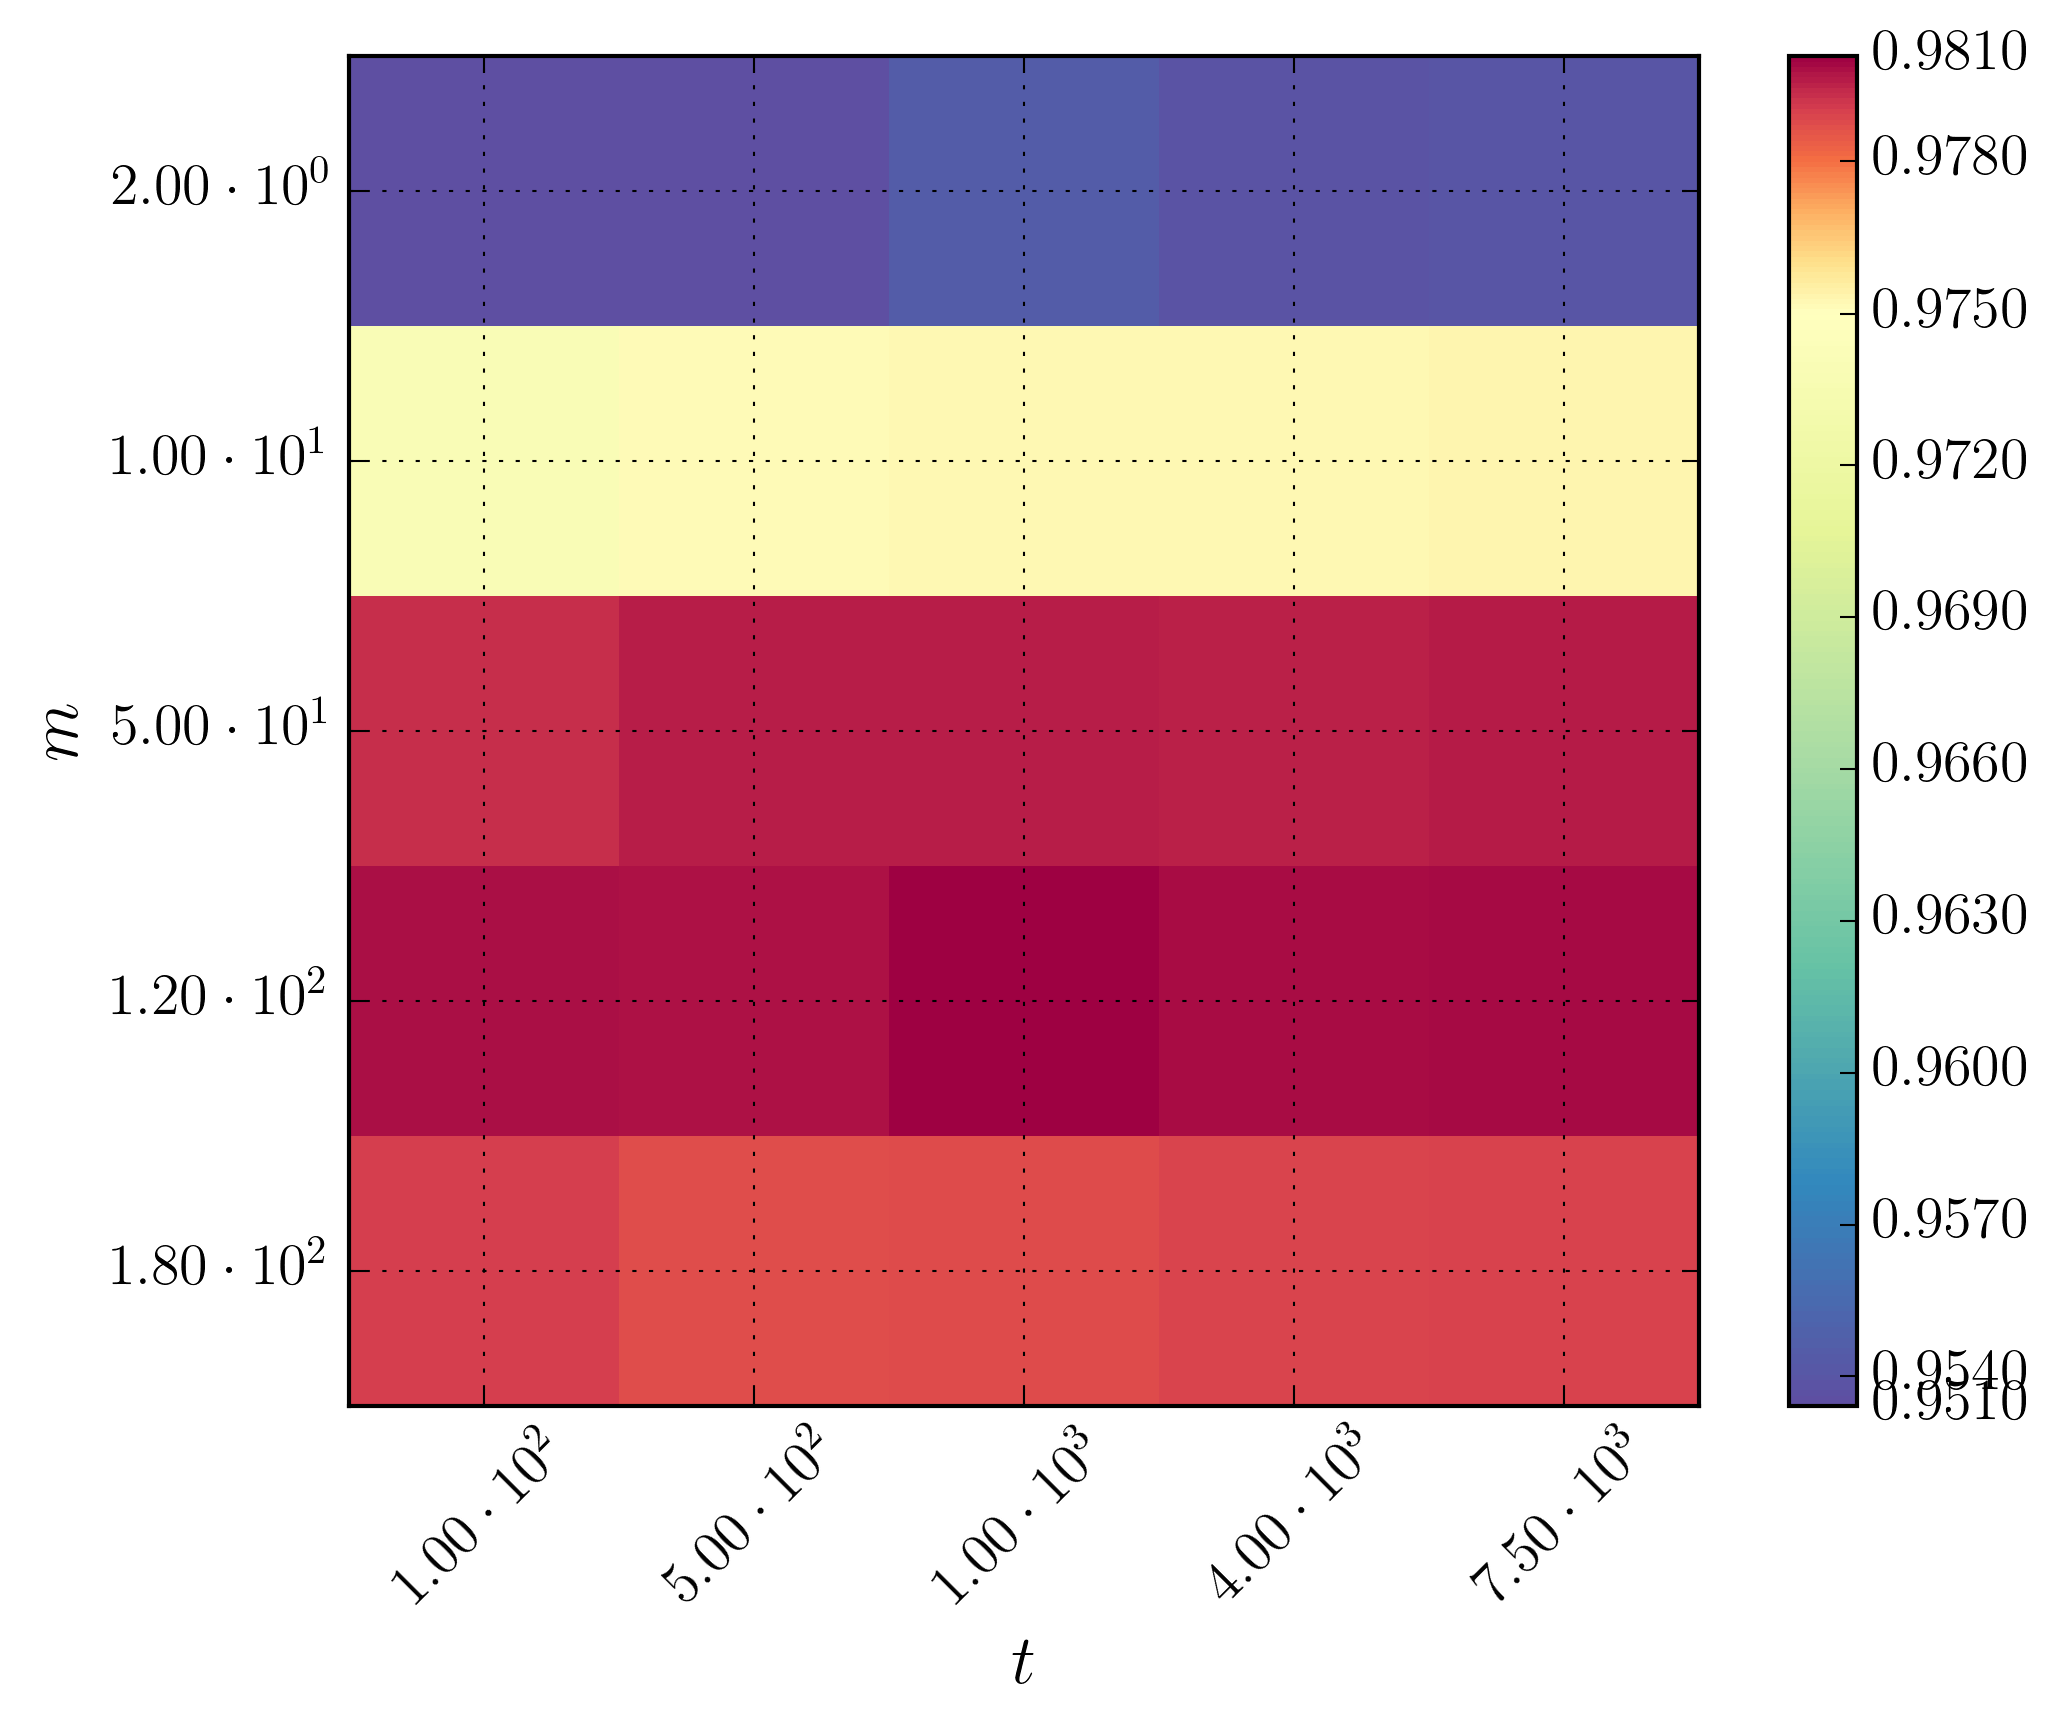
\includegraphics[width=0.49\textwidth,height=0.4\textwidth]{figures/gridsearch/rf/superclasses/rf-superclasses-01.png}}
\hfill
\subfigure{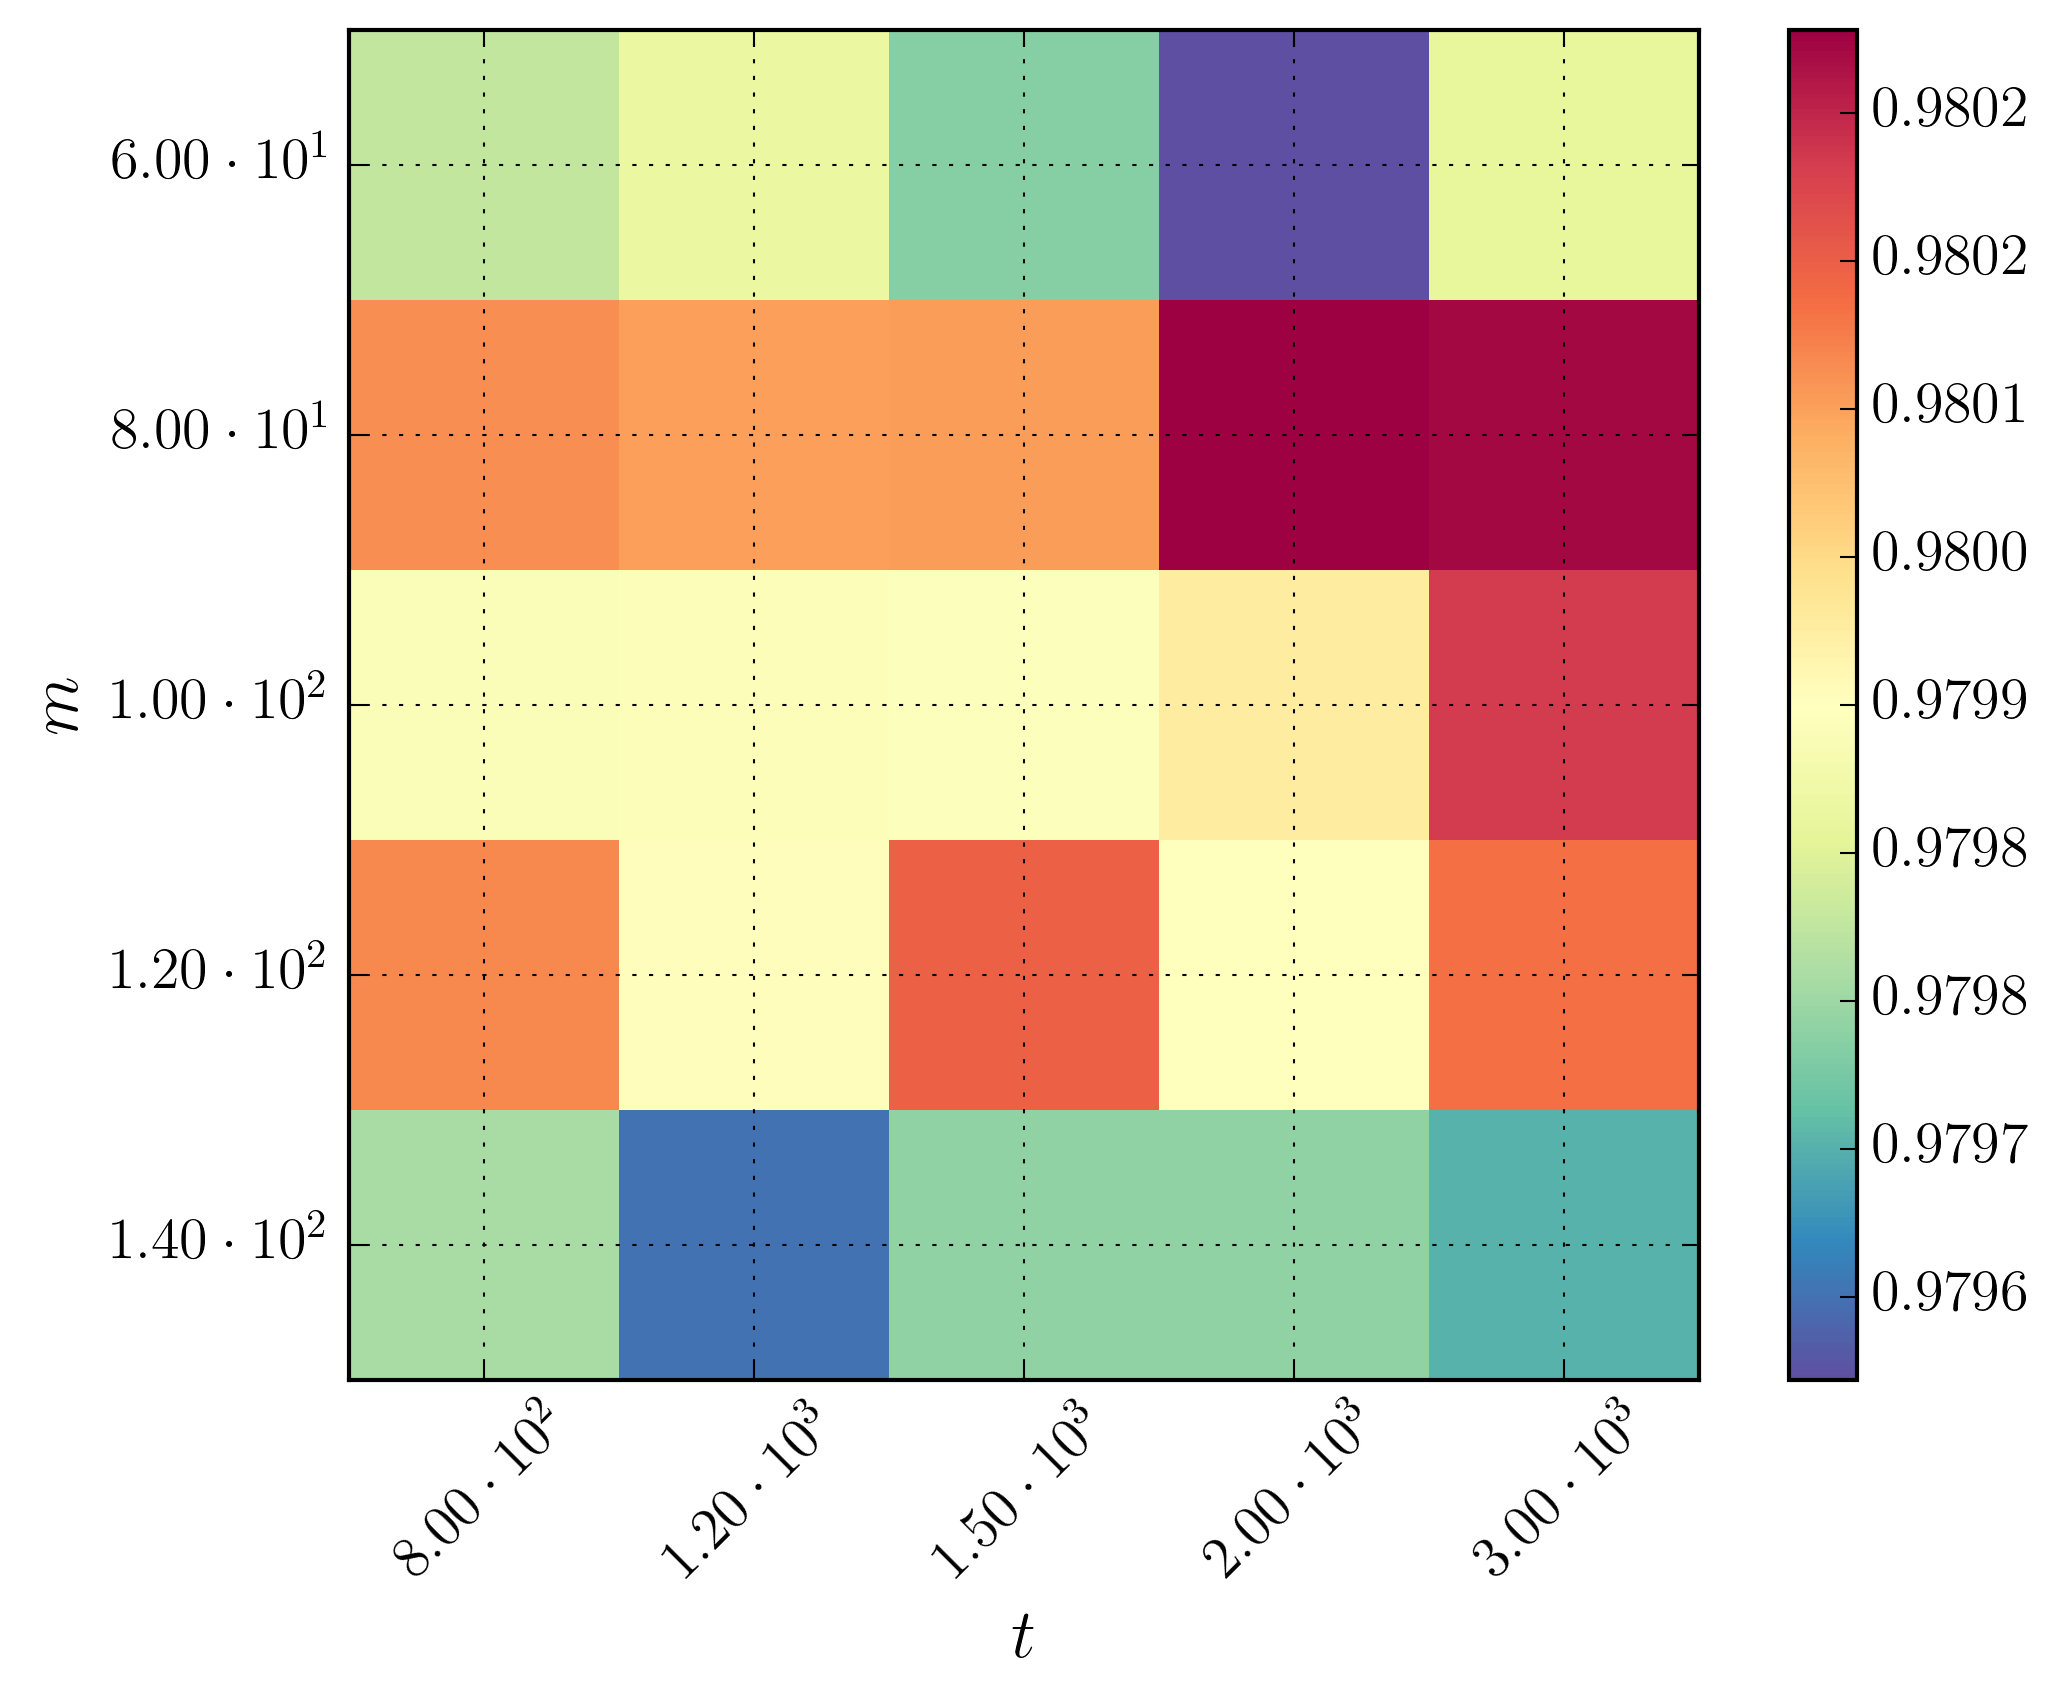
\includegraphics[width=0.51\textwidth,height=0.4\textwidth]{figures/gridsearch/rf/superclasses/rf-superclasses-02.png}}
\hfill
\subfigure{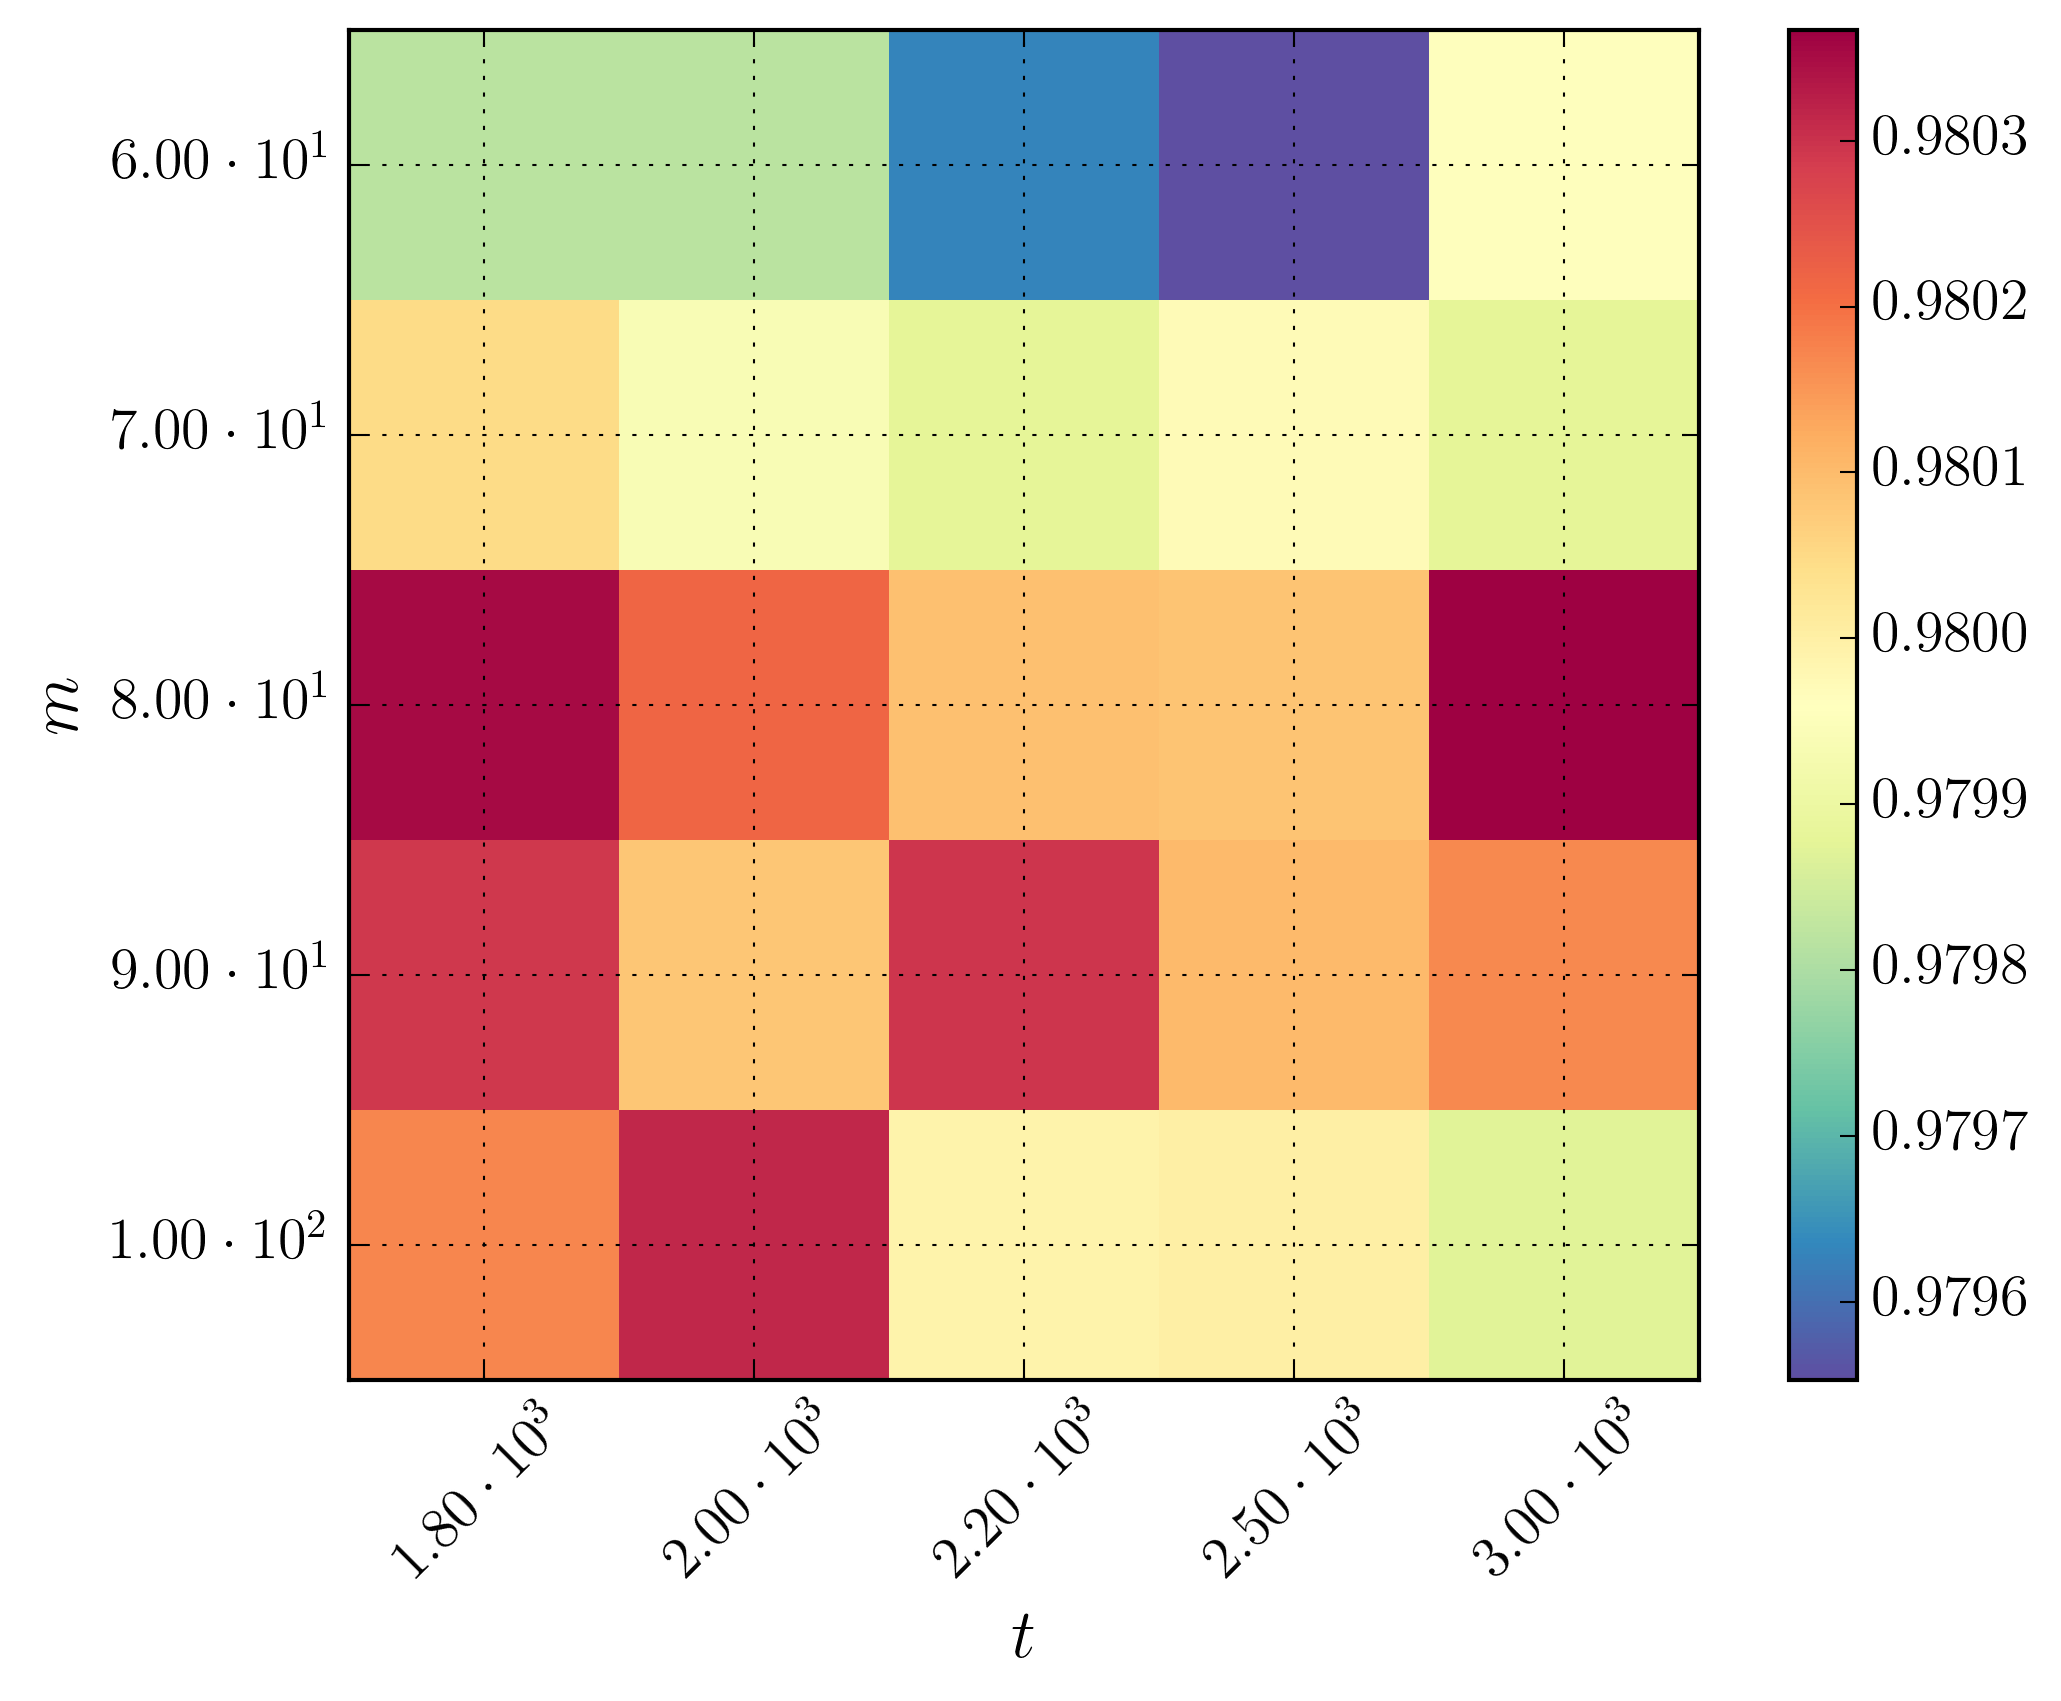
\includegraphics[width=0.49\textwidth,height=0.4\textwidth]{figures/gridsearch/rf/superclasses/rf-superclasses-03.png}}
\hfill
\subfigure{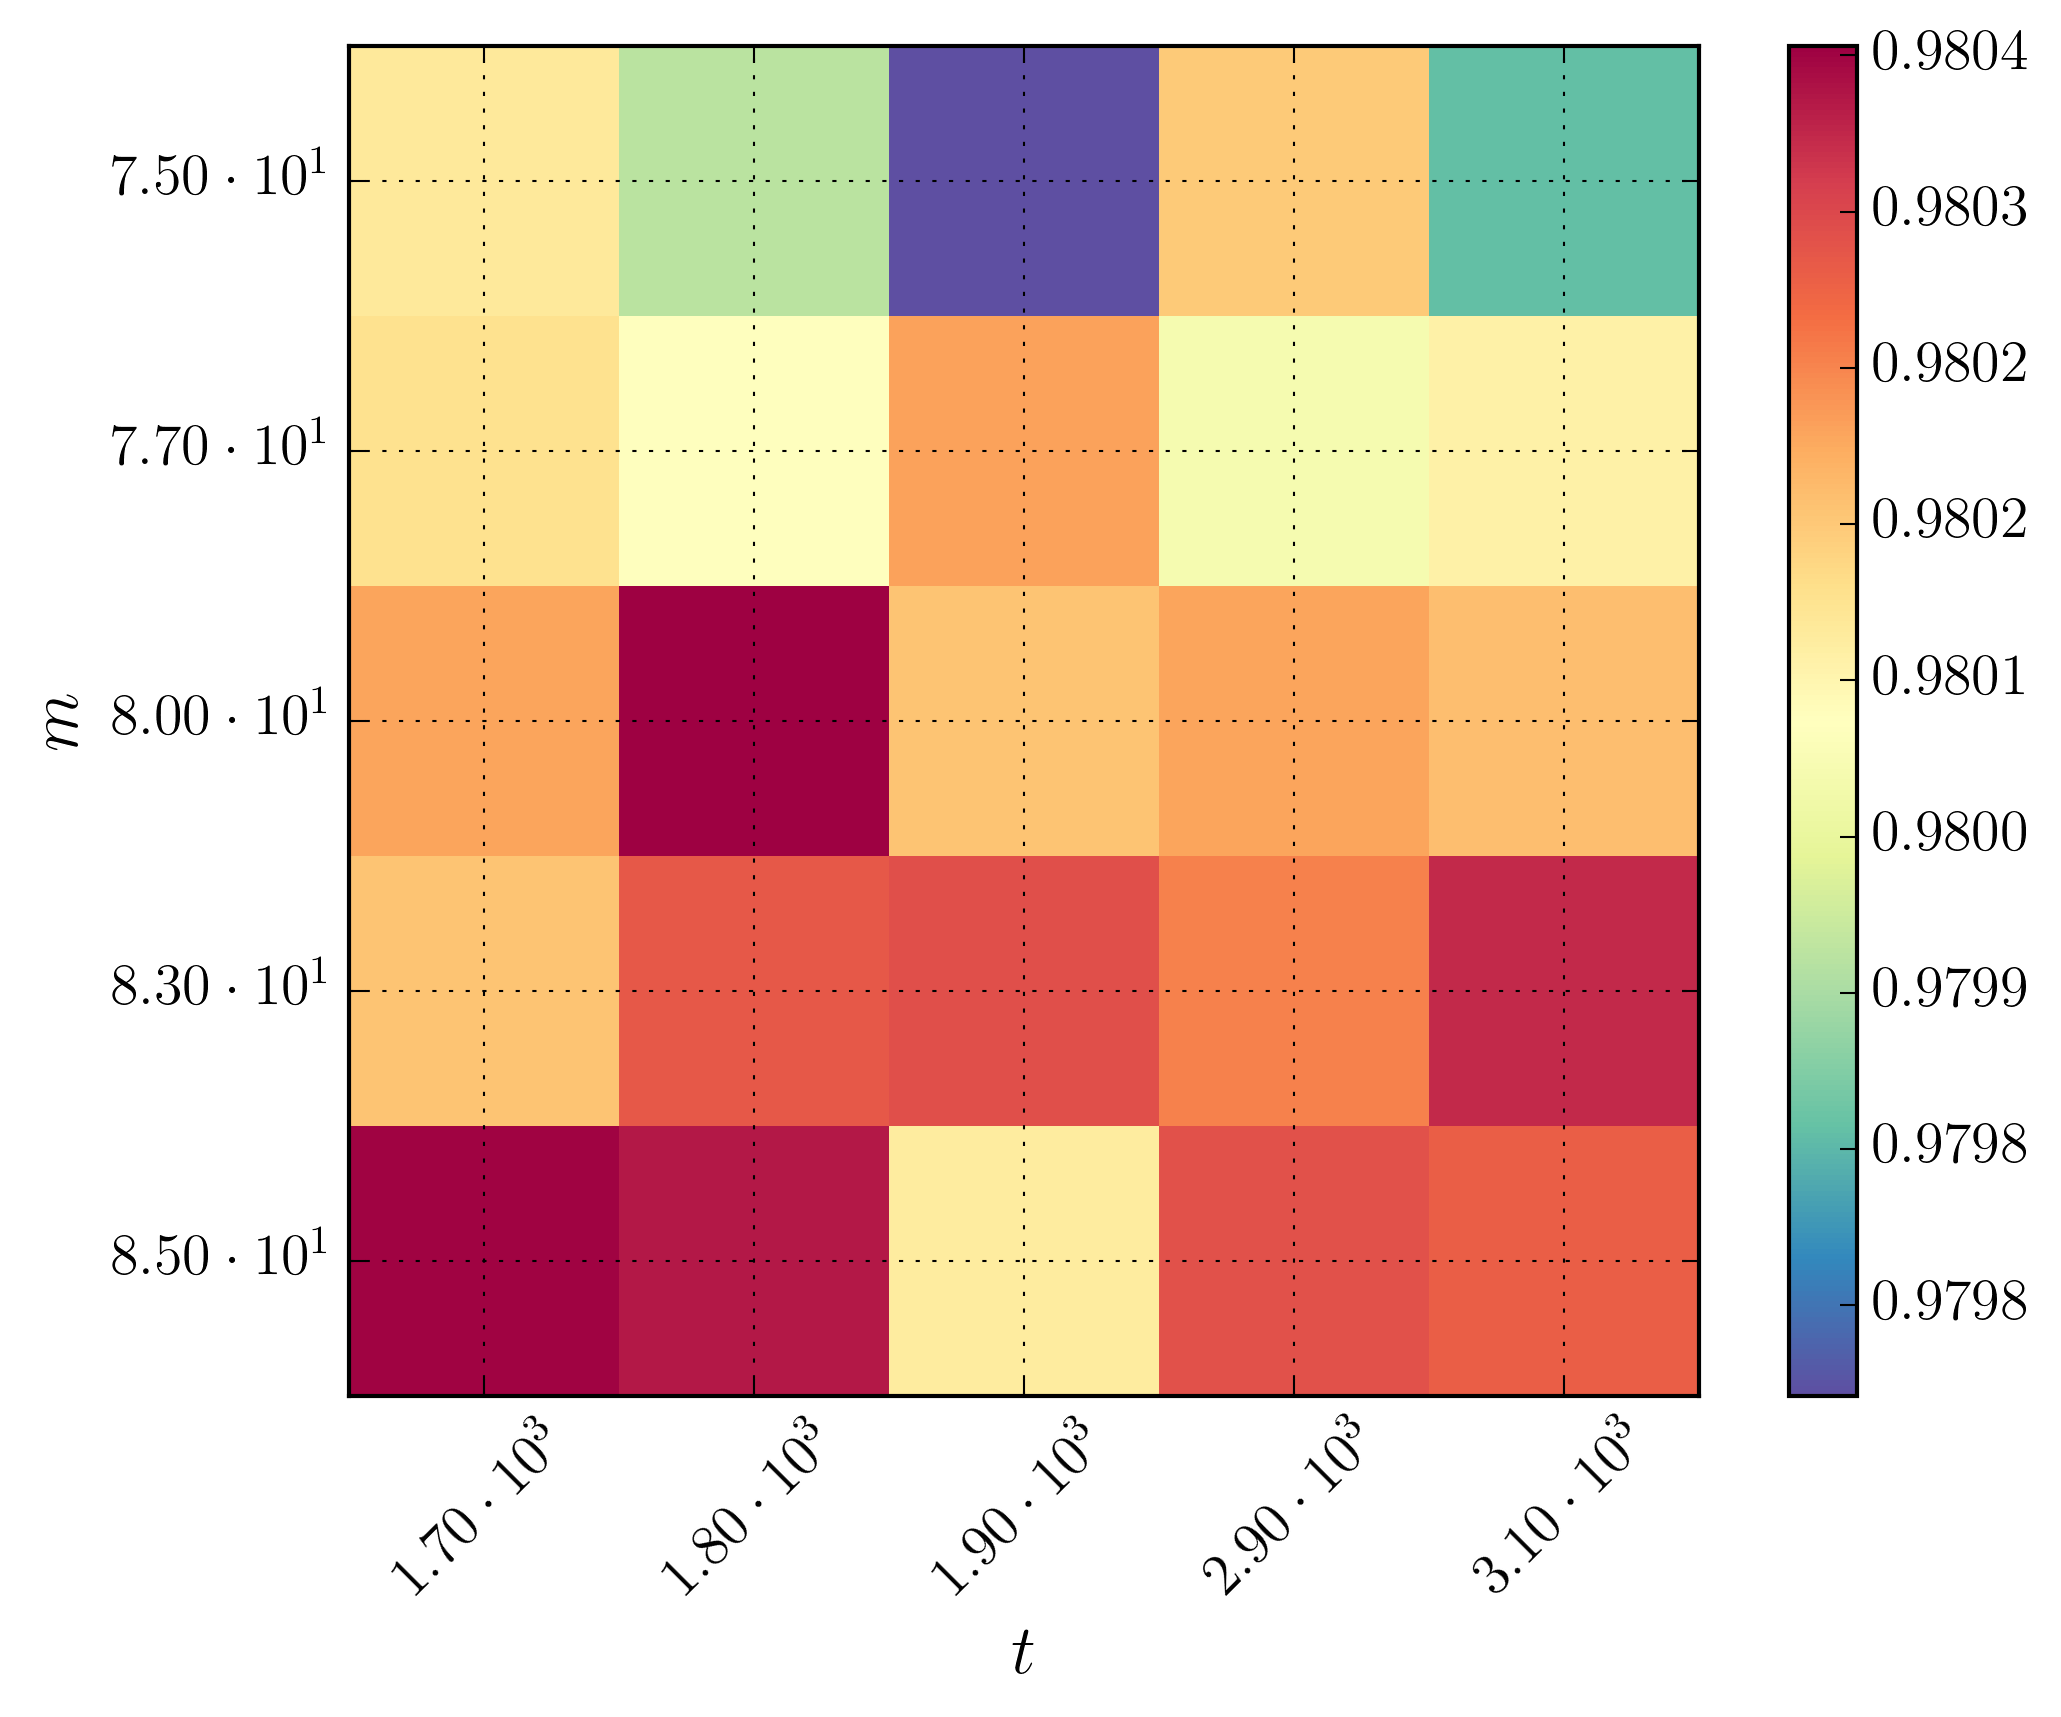
\includegraphics[width=0.51\textwidth,height=0.4\textwidth]{figures/gridsearch/rf/superclasses/rf-superclasses-04.png}}
\caption[Hyperparameter optimization for the Random Forest Classifier]{This figure shows the average, weighted $F_1$ score on the $m$-$t$-plane during the hyperparameter optimization for the Random Forest Classifier.$\cdots$}
\label{fig:gridsearch-rf-superclasses}
\end{figure}

\renewcommand{\arraystretch}{1.5}
\resizebox{\textwidth}{!}{
\begin{tabular}{c|ccccccccc|c}
\toprule
%& \multicolumn{8 }{c}{Predicted class} & & \\
%\hline
                   & BV        & CEPH       & DSCT      & EB         & LPV         & NoneVar    & QSO       & RRL        & T2CEPH   & $\Sigma $ \\
\hline
BV                 & {\bf 773} &            &           &     11     &      3      &      8     &      1    &            &          &     796   \\
CEPH               &     1     & {\bf 2226} &           &     18     &      2      &      3     &           &     31     &          &    2281   \\
DSCT               &           &            & {\bf 496} &      2     &             &     12     &           &      1     &          &     511   \\
EB                 &     7     &      7     &     2     & {\bf 3342} &     52      &     79     &      3    &     43     &     3    &    3538   \\
LPV                &     4     &      2     &           &     10     & {\bf 15945} &     32     &      1    &     1      &          &   15995   \\
NoneVar            &    23     &      1     &     4     &     35     &     72      & {\bf 4648} &      8    &            &          &    4791   \\
QSO                &           &            &           &      3     &      4      &     25     & {\bf 147} &     1      &          &     180   \\
RRL                &           &      9     &     7     &     31     &      2      &     7      &           & {\bf 4414} &          &    4470   \\
T2CEPH             &     1     &      15    &           &     19     &      5      &     3      &           &            & {\bf 78} &     121   \\
\bottomrule
Recall ($\%$)      &   97.11   &     97.59  &   97.06   &    94.46   &    99.69    &   97.02    &   81.67   &    98.75   &   64.46  &           \\
\hline
Precision ($\%$)   &   95.55   &     98.50  &   97.45   &    96.28   &    99.13    &   96.49    &   91.87   &    98.29   &   96.93  &           \\
\hline
$F_1$ score ($\%$) &   96.32   &     98.04  &   97.25   &    95.36   &    99.41    &   96.75    &   86.47   &    98.52   &   77.43  & 98.14 $\pm$ 0.07 \\
\bottomrule
\end{tabular}
}

% Hyperparameter optimization
% Add confusion matrix for main classes
% Add confusion matrix for subclasses
% Add feature importance for both

\chapter{Assessing Classification Performance for GAIA}

% Simulating GAIA time series
% Performance of the best classifier on GAIA data